\section{Evaluation}
\label{sec:eval}
\vspace{10pt}

\begin{comment}
~\bu{Suggestions for creating a first draft:
\begin{itemize}
\item In Section 4.1: When describing our experimental setup, refer to Table 1 to say we restrict our attention to these 6 VMs from AWS and only use num cores, memory, num replicas, and throughput as our independent variables. Our dependent variables are average read and write latencies.
\item Have a generic figure showing a YCSB client and one of our case studies with 3 replicas. 
\item For Sections 4.2-4.4, describe the graphs/tables being presented in some detail, identify any trends. Conclude each with a list of "Key insights"
\item Most figures and tables need more clarity on what exactly was the training set, for which VM the prediction is being done, etc. All figures need larger fonts on their axes, labels, etc. 
\item Replace R-squared with $R^2_{predicted}$. 
\end{itemize}

\end{comment}

\subsection{Methodology and Setup}
\vspace{10pt}

\begin{table}
\centering

\begin{tabular}{|r|l|c|r|l|} \hline
Instance name & Abbr.& \# cores&Memory&Network\\ \hline
m3.large & $VM_1$ & 2 & 7.5 GB & Moderate\\ \hline
m3.xlarge & $VM_2$ & 4 & 15 GB & Moderate\\ \hline
m3.2xlarge & $VM_3$ & 8 & 30 GB & High\\ \hline
r3.large & $VM_4$ & 2 & 15 GB & Moderate\\ \hline
r3.xlarge & $VM_5$ & 4 & 30.5 GB & Moderate\\ \hline
r3.2xlarge & $VM_6$ & 8 & 61 GB & High\\ \hline
\hline\end{tabular}
\caption{AWS instance types employed in our evaluation. }
\label{table:awstypes}
\end{table}

We carry out our evaluation on the EC2 public cloud offered by Amazon Web Services (AWS)~\cite{amazon-ec2}. We adapt our generic performance model from Section~\ref{sec:model} for three different types of latency-sensitive data-serving applications: (i) Redis (an in-memory open-source NoSQL key-value store)~\cite{redis}, (ii) Apache Cassandra (a NoSQL key-value store that can be configured for different consistency levels), and the popular MySQL ACID database~\cite{mysql}. We use the open-source Yahoo! Cloud Serving Benchmark (YCSB) as our workload generator~\cite{Cooper:2010:BCS:1807128.1807152}. We run the YCSB client on a m4.2xlarge EC2 instance running Ubuntu Linux 14.04. We monitor the system load average on the client machine to verify that the client is not the bottleneck during our tests.


  \begin{figure*}
    \centering
    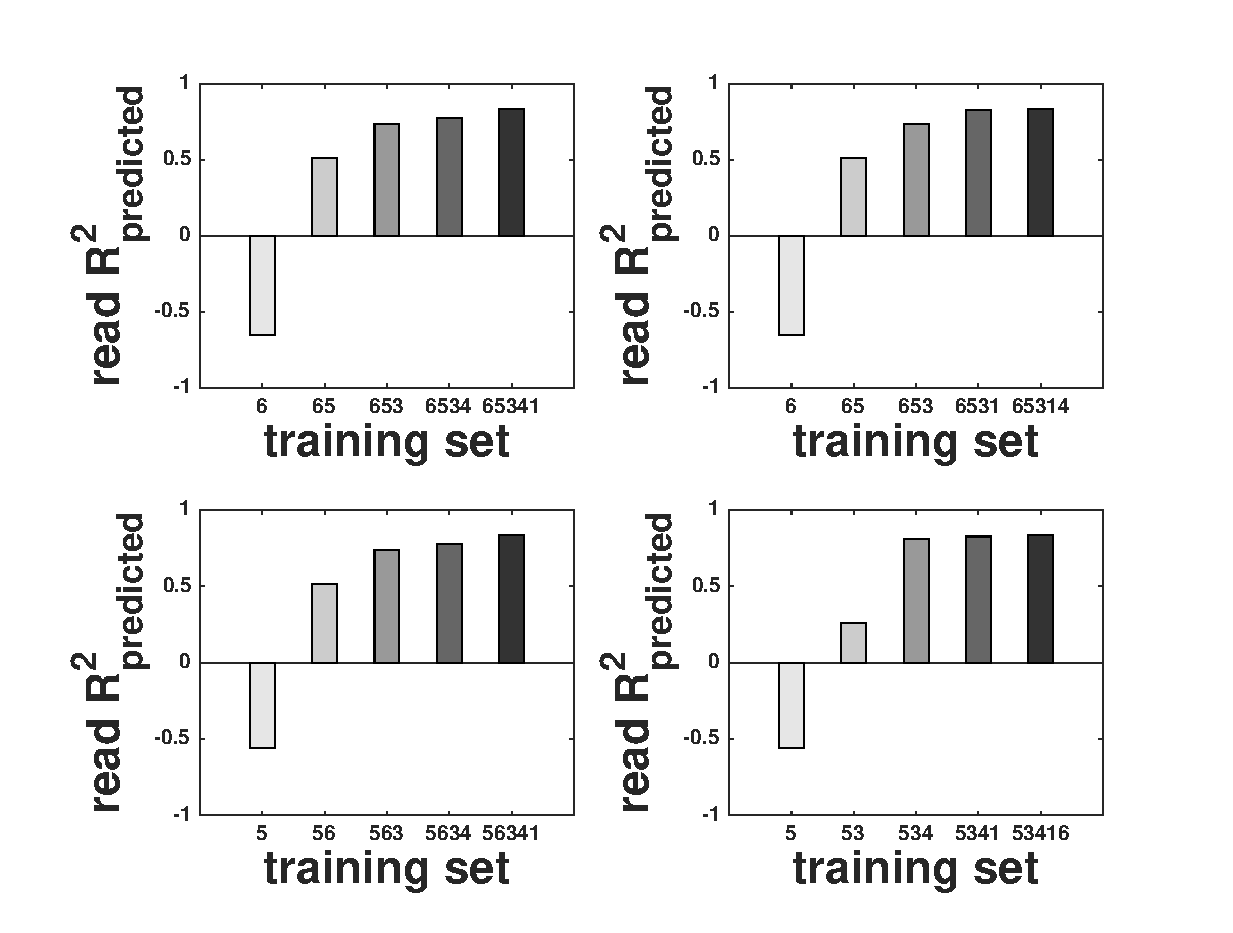
\includegraphics[scale = 0.4]{bar_read_avg_latency.eps}
    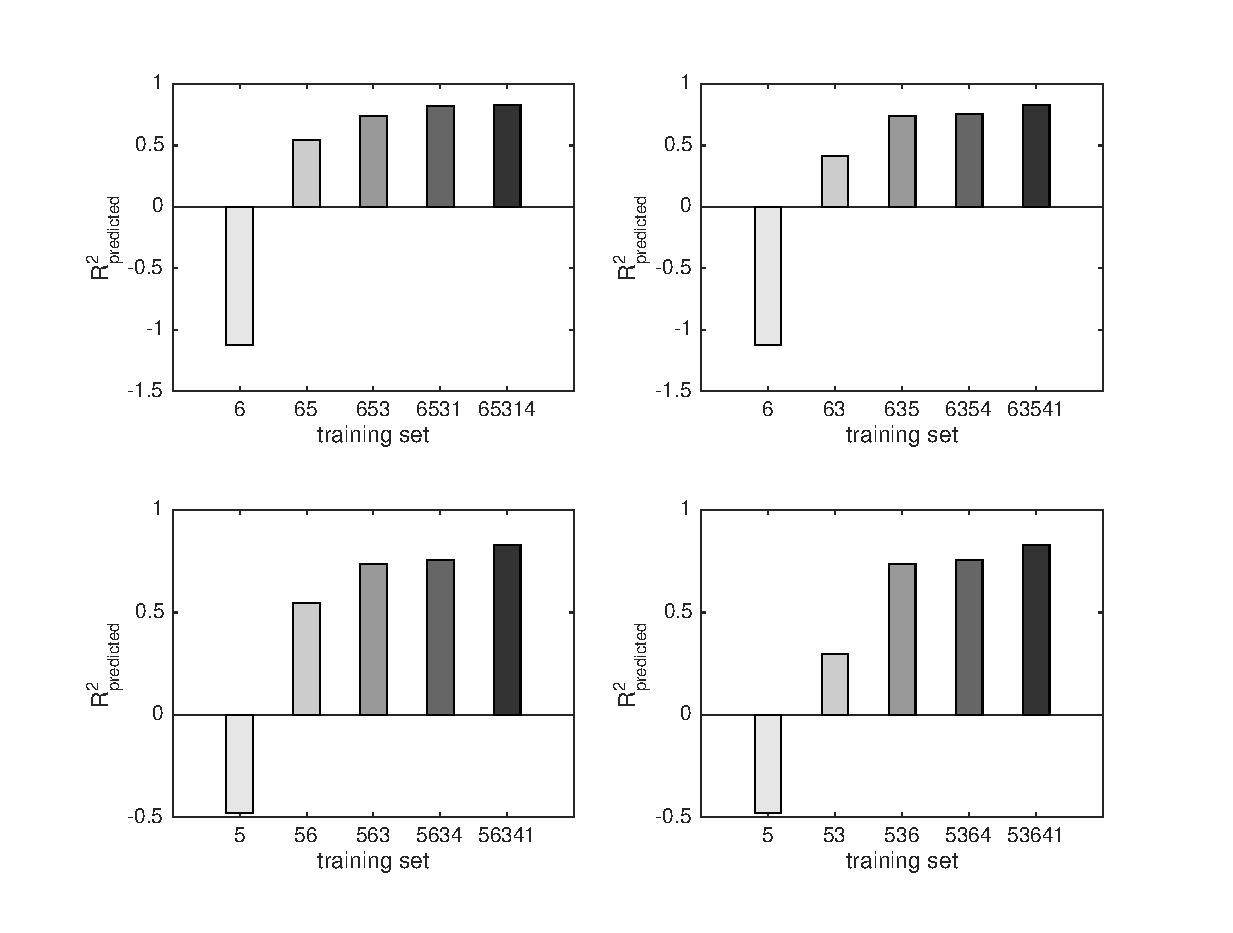
\includegraphics[scale = 0.4]{bar_write_avg_latency.eps}
    \caption{\textbf{Redis read and write $R^2_{predicted}$ vs training set.  We find that $R^2_{predicted}$ improves consistency with more diverse training sets for a wide range of training set choices supporting our basic hypothesis.}}
    \label{figure:redisbarreadwrite}
  \end{figure*}



We describe a subset of our overall results wherein for each experiment %case 
we load the concerned database with 1,000,000 records, each containing ten fields of 100 bytes each (the default). This amounts to an overall working set of about 1GB. Each experiment consists of subjecting the database to a particular thoughput and recording the average latency (separately for reads and writes). YCSB defines several standard workloads that we experiment with. We experiment with different workloads offered by YCSB and present a subset of our overall results - workload ``A'' for MySQL and ``B'' for Redis and Cassandra. Workload A has 50\% read and 50\% write requests and employs a uniform popularity distribution. Workload B has 95\% reads and 5\% writes, and  the popularity of requests is chosen based on a zipfian distribution. We repeat each experiment several times to achieve significantly tight confidence intervals. 
%Modeling and testing was done twice for each case study:  once for read latency and once for write latency.  The ratio of the number of write operations to read operations is another potential independent variable.  For our study, this was fixed as all testing was done with 95\%/5\% read/write.
%  Three test runs were done for each throughput and instance type to check the reproducibility of results.
Amazon EC2 is hosted in multiple geographic regions around the world, and multiple zones within each region.  We create our testing client and servers within the same region (us-west) and availability zone (2b) to minimize the effect of network latency. Finally, we pick all VMs having individual CPUs offering the same clock rate. 

 %To ensure that CPU count and memory can be safely considered independent variables (an important assumption of linear regression, recall from Section~\ref{sec:model}), 
We select the VM instances listed in Table~\ref{table:awstypes}.  
There are three instances from the M3 group (standard) and three from the R3 group (memory optimized).  The memory/CPU ratio is the same within each group, with the R3 group having twice the memory/cpu as the M3 group.  A more extensive study with more instances would allow the use of more independent variables in the model, e.g., including testing of instances in the C3 group (compute optimized), which have half as much memory/CPU as M3.

With the above choices, the measurements and modeling reported here effectively only employ a subset of all the independent variables listed in Section~\ref{sec:model}: number of CPU cores, throughput, number of replicas, and read-write ratio. In particular, our working set of 1GB fits fully within any of the chosen VMs, effectively rendering memory capacity moot as a predictive variable. In our more general experiments, however, we explore a much larger set of workload choices. 

\begin{figure*}
\subfloat[]{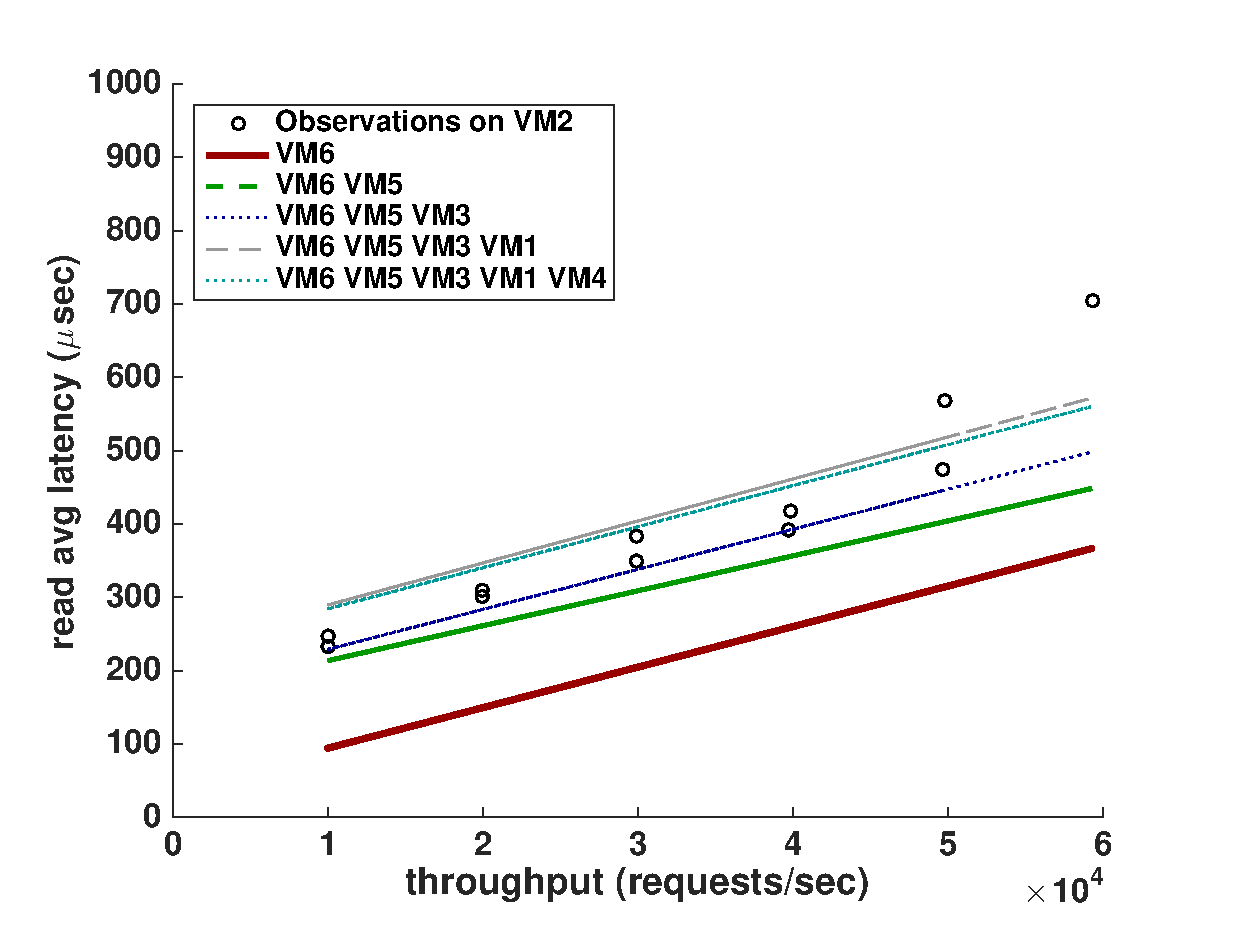
\includegraphics[width=0.5\textwidth]{fit_read_avg_latency_r3_2x_r3_x_m3_2x_m3__r3__m3_x.eps}} 
\subfloat[]{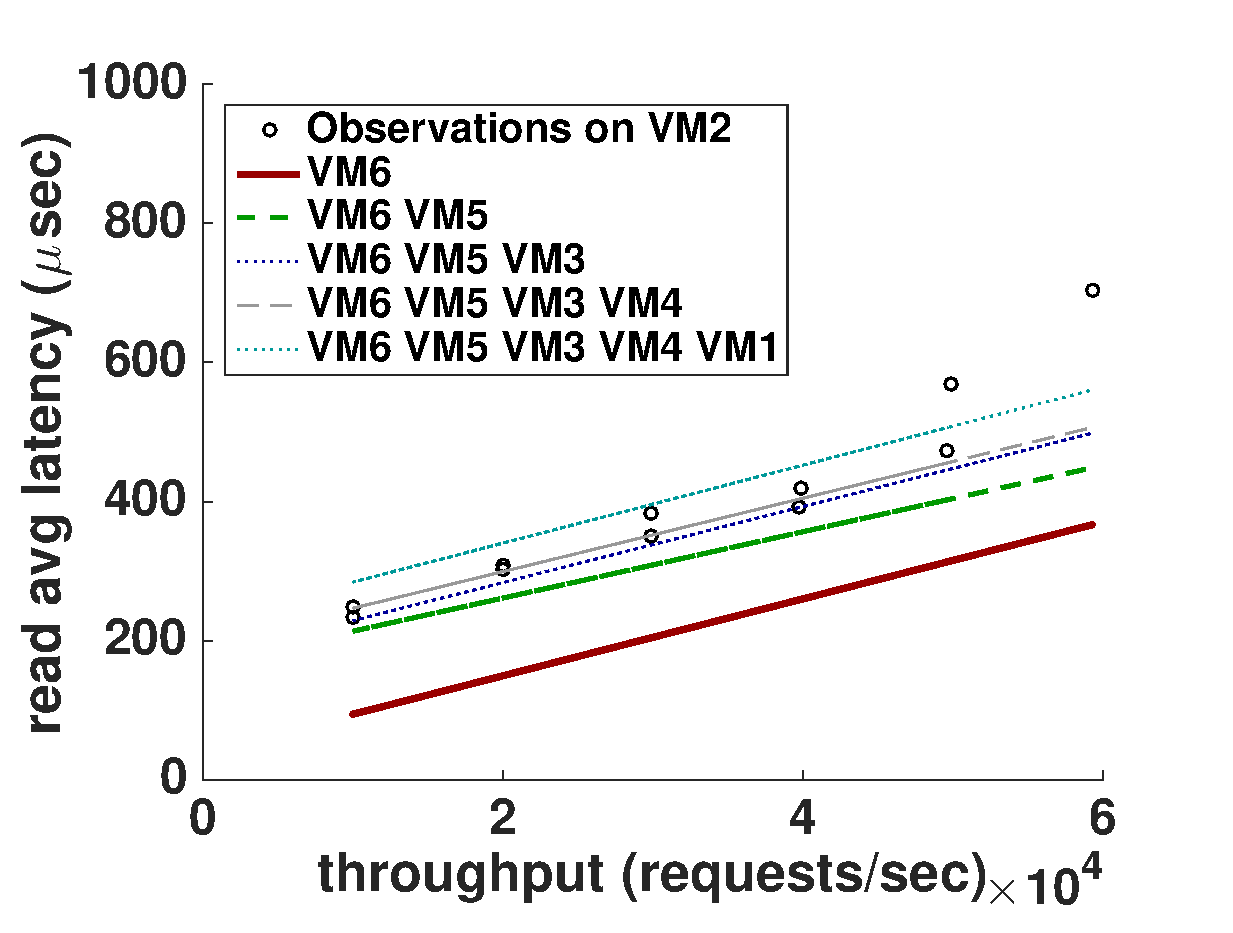
\includegraphics[width=0.5\textwidth]{fit_read_avg_latency_r3_2x_r3_x_m3_2x_r3__m3__m3_x.eps}}\\
\subfloat[]{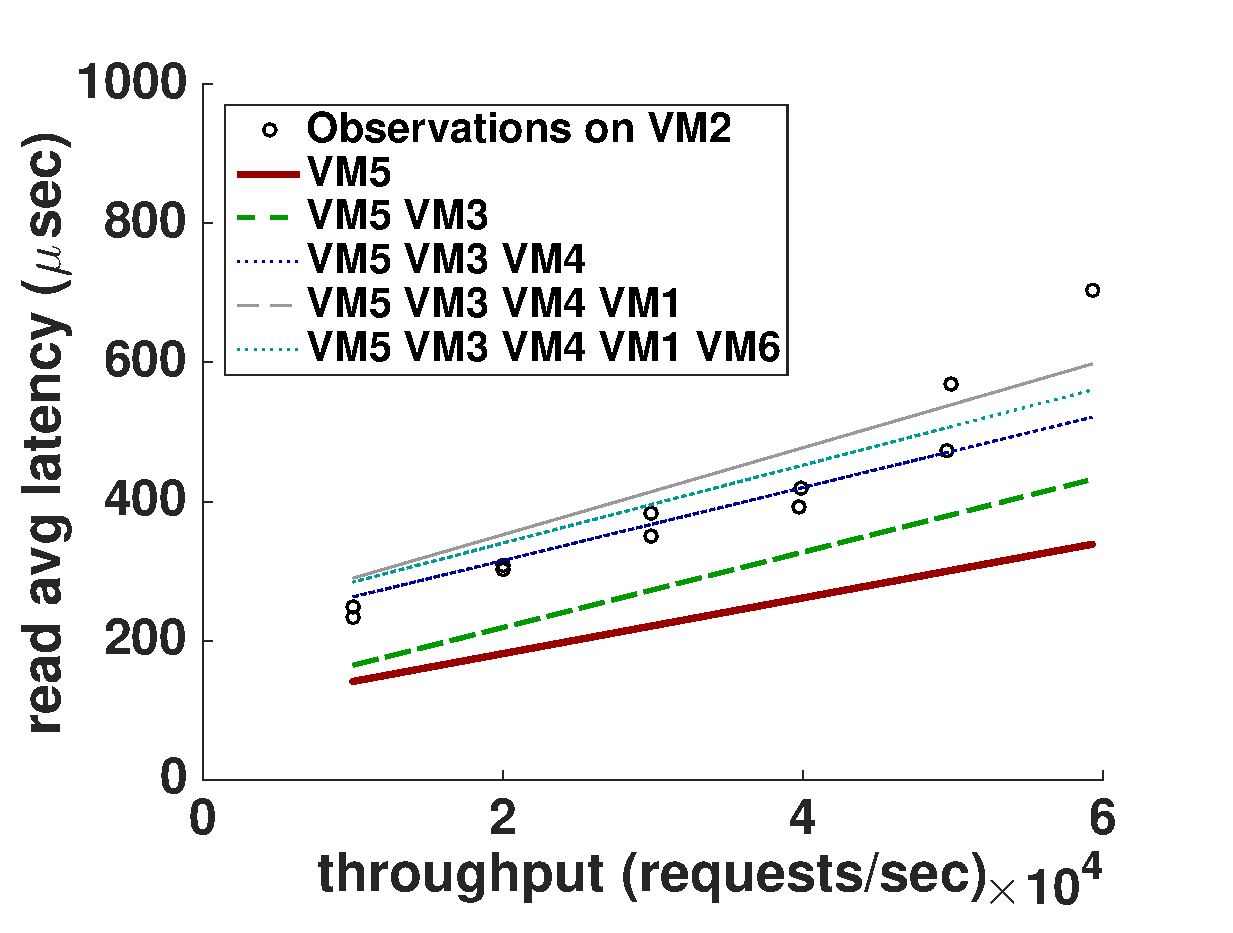
\includegraphics[width=0.5\textwidth]{fit_read_avg_latency_r3_x_m3_2x_r3__m3__r3_2x_m3_x.eps}}
\subfloat[]{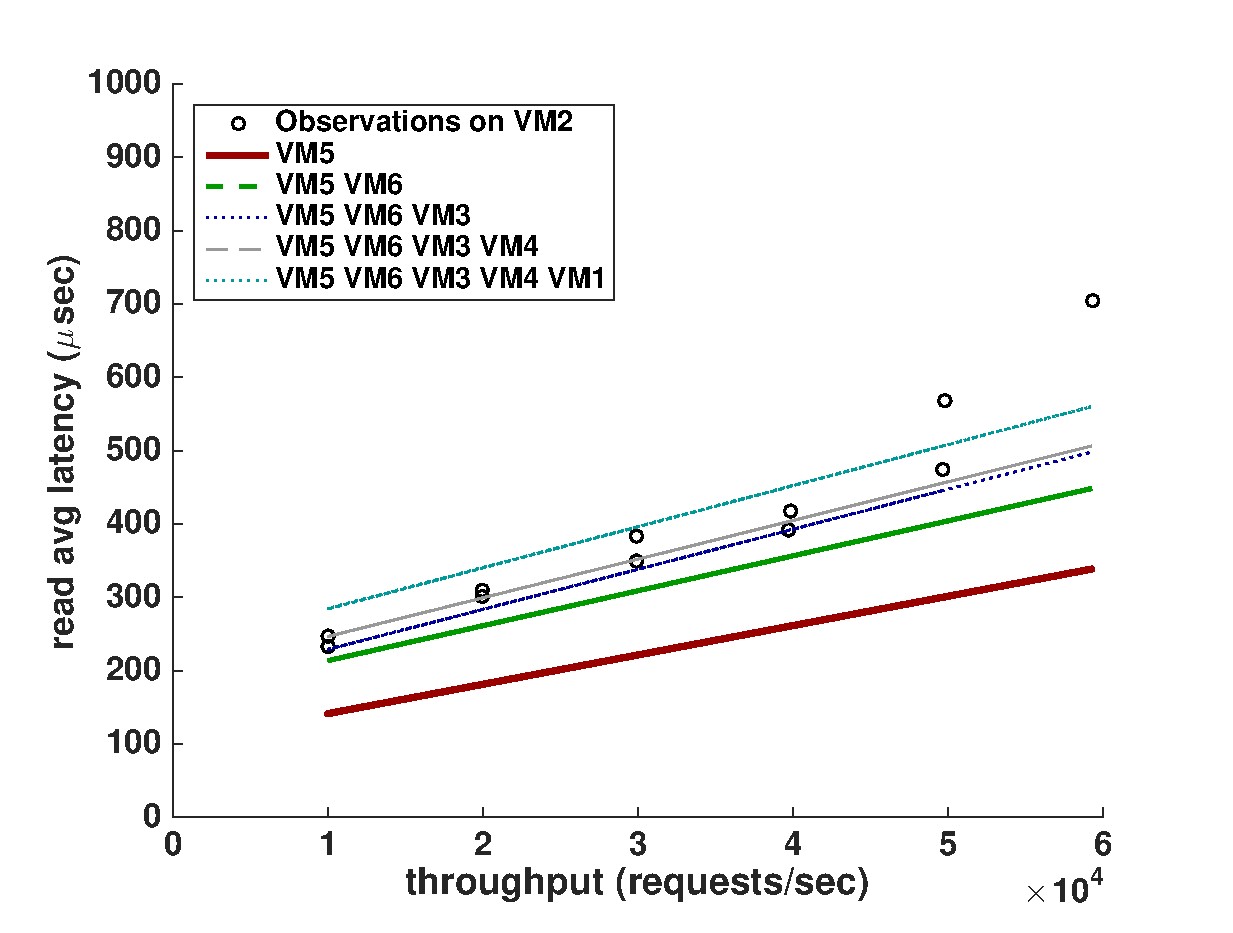
\includegraphics[width=0.5\textwidth]{fit_read_avg_latency_r3_x_r3_2x_m3_2x_r3__m3__m3_x.eps}} 
\caption{Prediction of Redis read latency on $VM_2$ compared for model calibration using a variety of training sets ranging in size from 1 to 5 VM types. }
\label{figure:redisfitread}
\end{figure*}

\begin{table}
\centering
\caption{Redis $R_{predicted}^2$ for $VM_1$}
\begin{tabular}{|r|r|l|} \hline
reads&writes&Training Set\\ \hline
-1.92604 & -1.12245  & VM6 \\ \hline 
0.0845781 &  0.547705 & VM6 VM5 \\ \hline 
0.1796 &  0.738969 & VM6 VM5 VM3 \\ \hline 
0.377601 & 0.821984  & VM6 VM5 VM3 VM4 \\ \hline 
0.475624 &  0.827944 & VM6 VM5 VM3 VM4 VM2 \\ \hline 
\hline\end{tabular}
\label{table:redis1}
% \end{table}

% \begin{table}
\centering
\caption{Redis $R_{predicted}^2$ for $VM_2$}
\begin{tabular}{|r|r|l|} \hline
reads&writes&Training Set\\ \hline
-0.648416 & -1.12245  & VM6 \\ \hline 
0.51488 &  0.41527 & VM6 VM5 \\ \hline 
0.738979 & 0.738969  & VM6 VM5 VM3 \\ \hline 
0.832156 &  0.756578 & VM6 VM5 VM3 VM1 \\ \hline 
0.837957 & 0.827944  & VM6 VM5 VM3 VM1 VM4 \\ \hline 
\hline\end{tabular}
\label{table:redis2}
% \end{table}

% \begin{table}
\centering
\caption{Redis $R_{predicted}^2$ for $VM_2$}
\begin{tabular}{|r|r|l|} \hline
reads&writes&Training Set\\ \hline
-0.559516 & -0.47657  & VM5 \\ \hline 
0.260701 &  0.547705 & VM5 VM3 \\ \hline 
0.738979 &  0.738969 & VM5 VM3 VM6 \\ \hline 
0.776002 & 0.756578  & VM5 VM3 VM6 VM4 \\ \hline 
0.837957 & 0.827944  & VM5 VM3 VM6 VM4 VM1 \\ \hline 
\hline\end{tabular}
\label{table:redis3}
% \end{table}

% \begin{table}
\centering
\caption{Redis $R_{predicted}^2$ for $VM_2$}
\begin{tabular}{|r|r|l|} \hline
reads&writes&Training Set\\ \hline
-0.559516 & -0.47657  & VM5 \\ \hline 
0.51488 & 0.29636  & VM5 VM6 \\ \hline 
0.738979 & 0.738969  & VM5 VM6 VM3 \\ \hline 
0.776002 & 0.756578  & VM5 VM6 VM3 VM4 \\ \hline 
0.837957 & 0.827944  & VM5 VM6 VM3 VM4 VM1 \\ \hline 
\hline\end{tabular}
\label{table:redis4}
\end{table}
 





\subsection{Case Study 1: Redis}
\label{sec:redis}
\vspace{10pt}

Redis is an open-source, key/value NoSQL database.  Redis is in-memory and,  therefore,  very fast.  Redis also optionally supports persistence, so unlike memcached it can be used as a primary database or as a cache.
We deploy Redis on AWS using Amazon ElastiCache, a web service that abstracts the deployment and administration of the OS and database software.  Elasticache supports up to five read replicas of the primary database. We report results with a single replica here.




For a VM type on which we wish to predict Redis performance, we choose training sets of different sizes from among the remaining VM types. We present sample results for predicting performance on $VM_2$ using different subsets of the remaining VMs in Tables~\ref{table:redis1}-\ref{table:redis4}. We find that each time we add a new instance type to the training set, $R^2_{predicted}$ does improve for both read and write latency. Generally, we observe that a training set of only 3 VM types appears to offer high accuracy with further additions offering relatively low gains. This bodes well for cost-efficacy of our model calibration approach - instead of having to calibrate its performance model for dozens of VM types (with associated costs), a tenant may be able to achieve comparable model accuracy using a much smaller set. 



We employ an alternate representation of the above findings in Figures~\ref{figure:redisbarreadwrite}, wherein we plot histograms of $R^2_{predicted}$ to highlight the improvement brought about with adding more diverse VMs. The x-axis is labeled with numbers for the VM types making up a particular training set. 

Finally, Figure~\ref{figure:redisfitread} allows us to compare the linear fits offered by several training sets and offers visual evidence of improvement in model accuracy with increase in the size of the training set. Figure~\ref{figure:redisfitwrite} presents a similar comparison for predictions of write latency. 



\begin{comment}

\begin{figure}[htbp]
\centering	
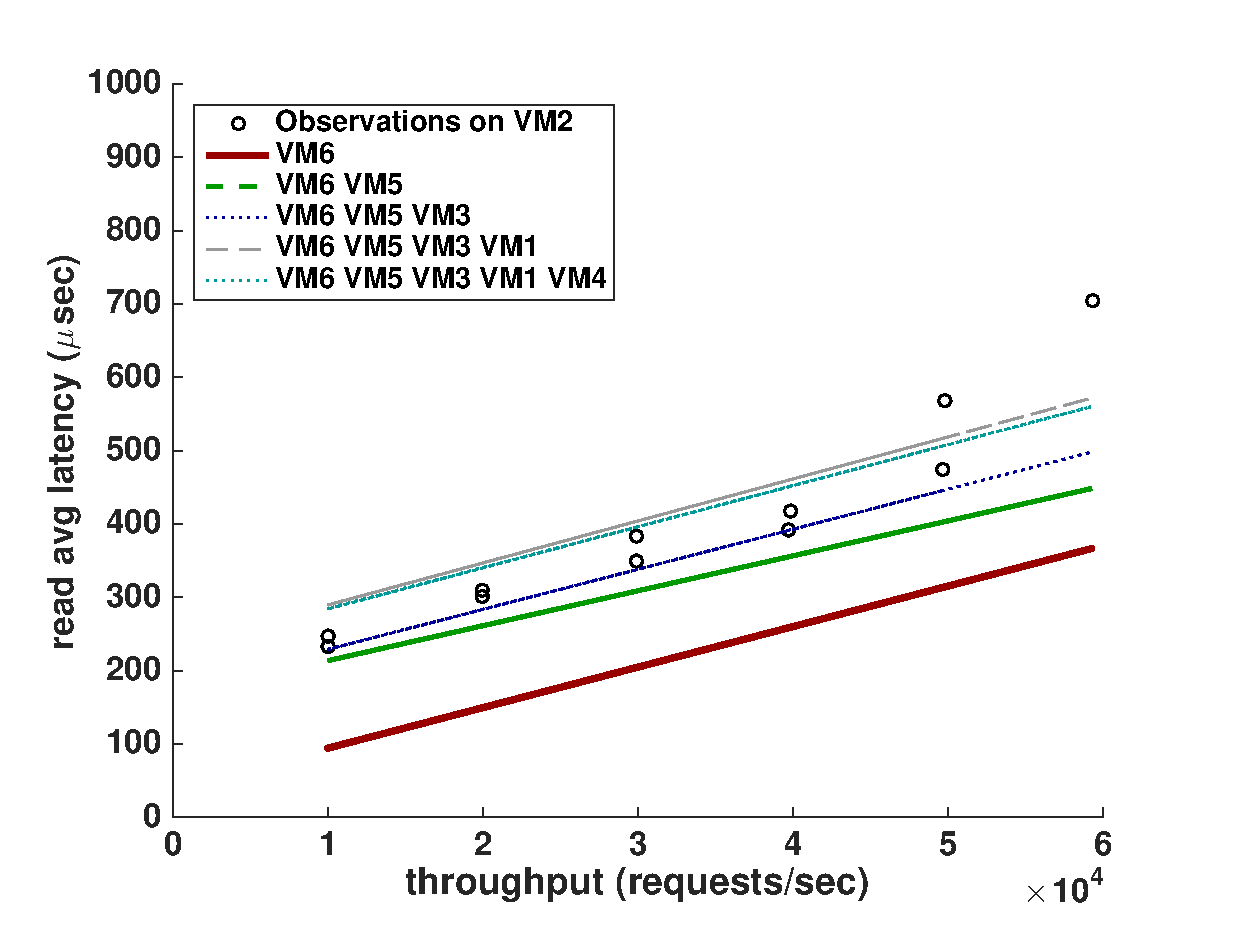
\includegraphics[width=0.45\textwidth]{fit_read_avg_latency_r3_2x_r3_x_m3_2x_m3__r3__m3_x.eps}
\caption{Redis average read latency vs throughput. ~\bu{TODO: cleanup plot formatting; make the numbers on the axes larger, label both the axes, use darker colors, move the box with names of providers to the top-left part of the graph.}}
\label{figure:redisbarread}
\end{figure}

\begin{figure}[htbp]
\centering	
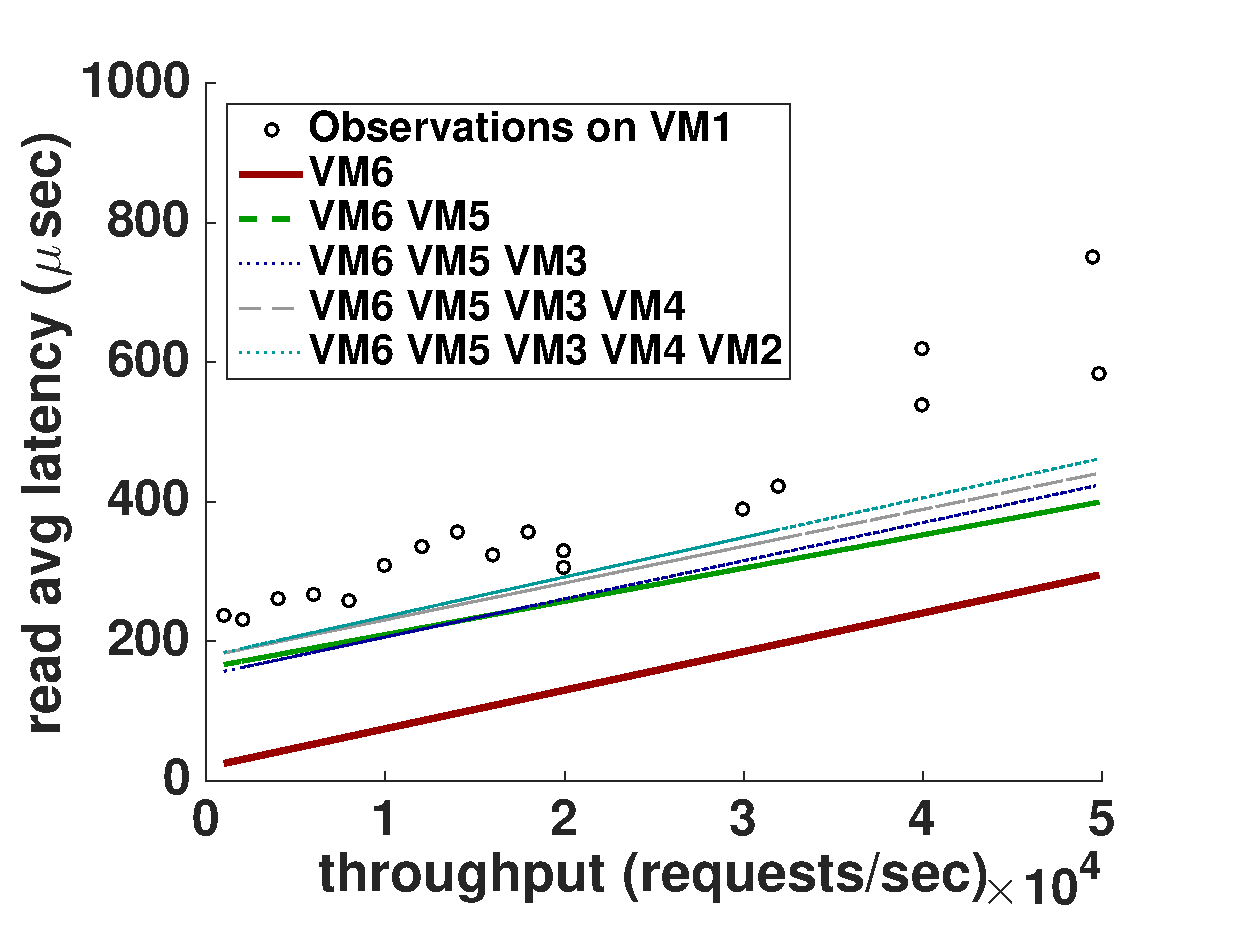
\includegraphics[width=0.45\textwidth]{fit_read_avg_latency_r3_2x_r3_x_m3_2x_r3__m3_x_m3_.eps}
\caption{Redis average read latency vs throughput. ~\bu{TODO: cleanup plot formatting; make the numbers on the axes larger, label both the axes, use darker colors, move the box with names of providers to the top-left part of the graph.}}
\label{figure:redisbarread}
\end{figure}

\begin{figure}[htbp]
\centering	
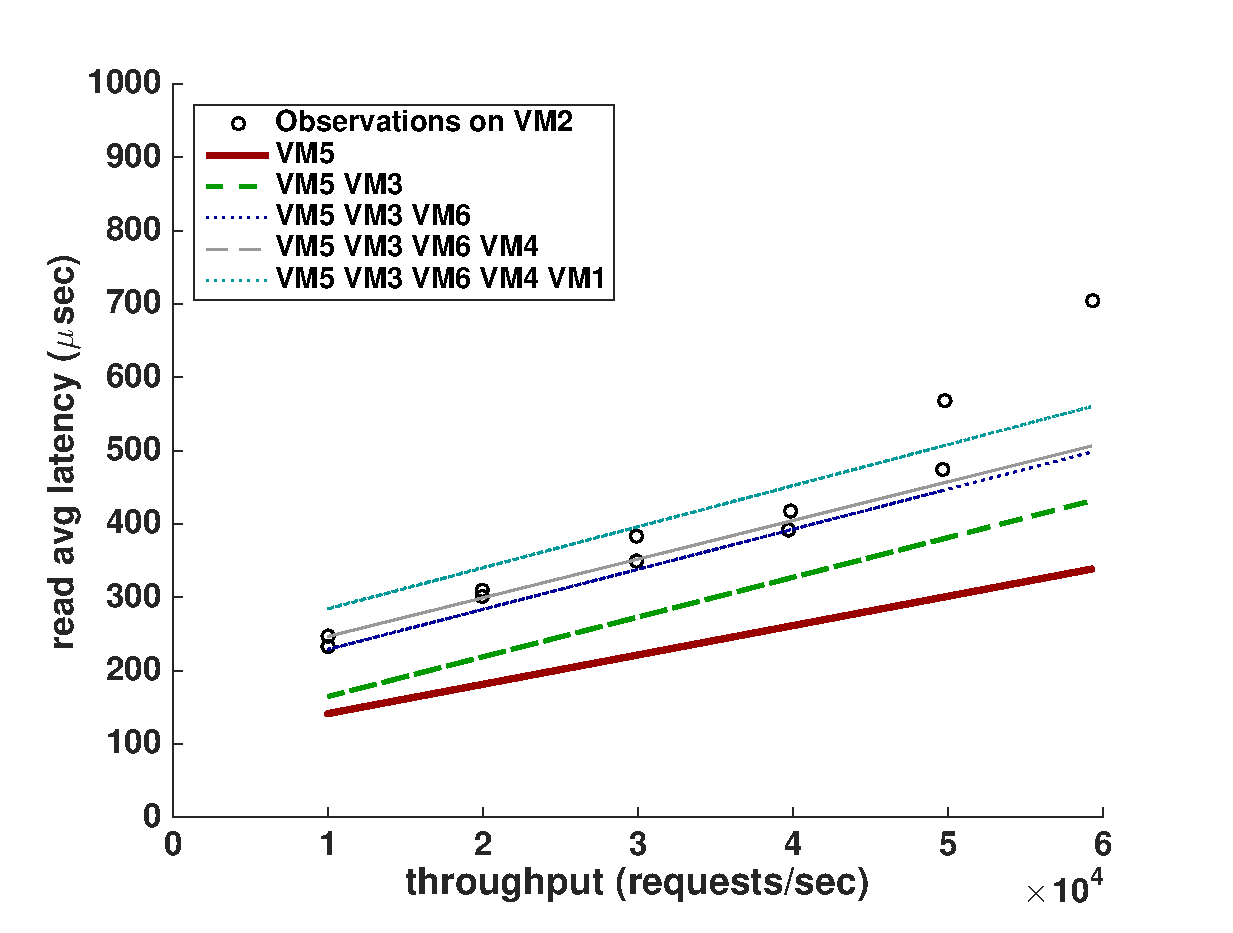
\includegraphics[width=0.45\textwidth]{fit_read_avg_latency_r3_x_m3_2x_r3_2x_r3__m3__m3_x.eps}
\caption{Redis average read latency vs throughput. ~\bu{TODO: cleanup plot formatting; make the numbers on the axes larger, label both the axes, use darker colors, move the box with names of providers to the top-left part of the graph.}}
\label{figure:redisbarread}
\end{figure}

\begin{figure}[htbp]
\centering	
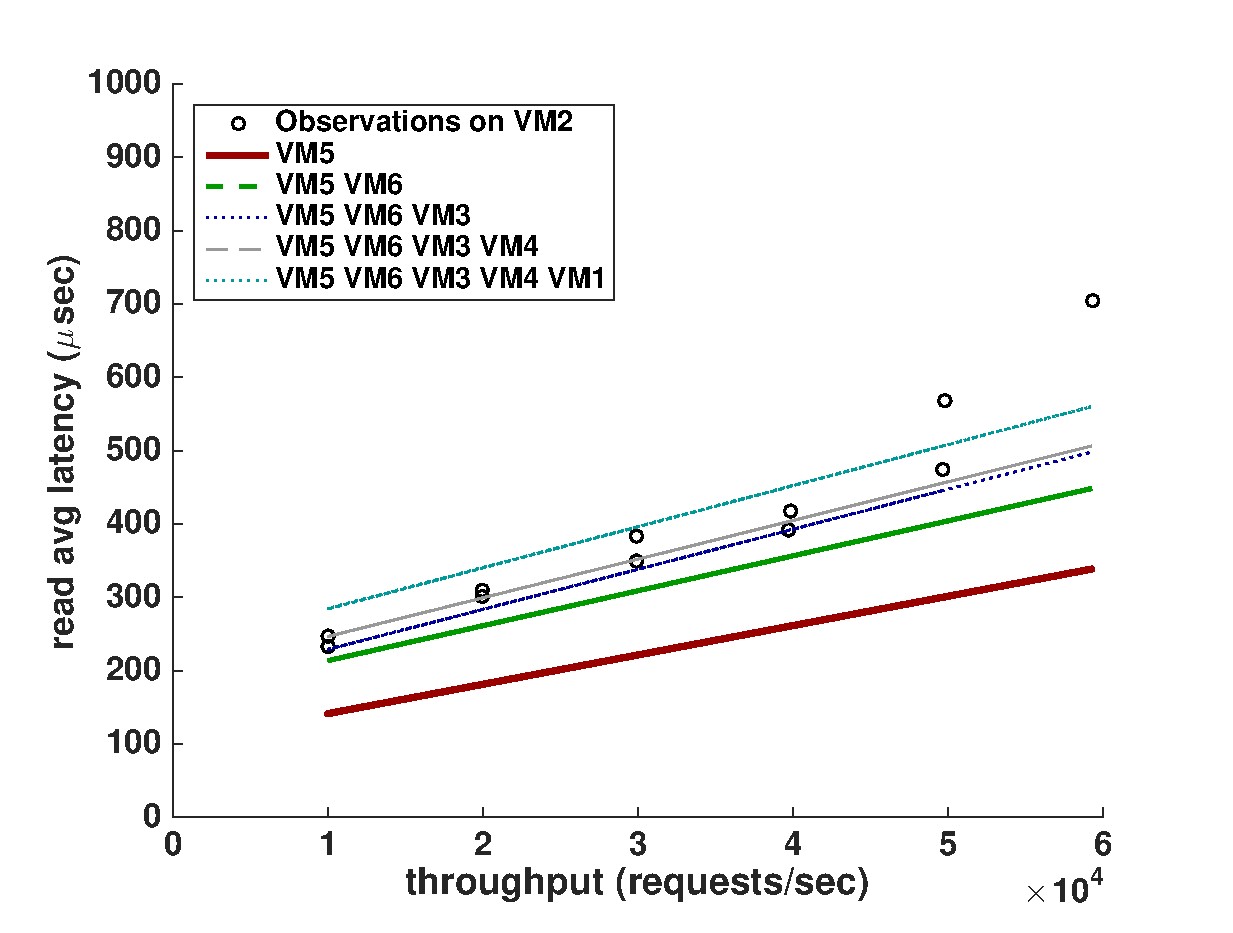
\includegraphics[width=0.45\textwidth]{fit_read_avg_latency_r3_x_r3_2x_m3_2x_r3__m3__m3_x.eps}
\caption{Redis average read latency vs throughput. ~\bu{TODO: cleanup plot formatting; make the numbers on the axes larger, label both the axes, use darker colors, move the box with names of providers to the top-left part of the graph.}}
\label{figure:redisbarread}
\end{figure}

%\begin{figure}[t]
%\twobytwofig{fit_read_avg_latency_r3_2x_r3_x_m3_2x_m3__r3__m3_x.eps}{}
%{fit_read_avg_latency_r3_2x_r3_x_m3_2x_r3__m3_x_m3_.eps}{}
%{fit_read_avg_latency_r3_x_m3_2x_r3_2x_r3__m3__m3_x.eps}{}
%{fit_read_avg_latency_r3_x_r3_2x_m3_2x_r3__m3__m3_x.eps}{}
%\caption{Profiles of Various Server Applications}
%\label{fig:redisread}
%\end{figure}

\end{comment}


%%%%%%%%%%%%

\begin{comment}

\begin{figure}[htbp]
\centering	
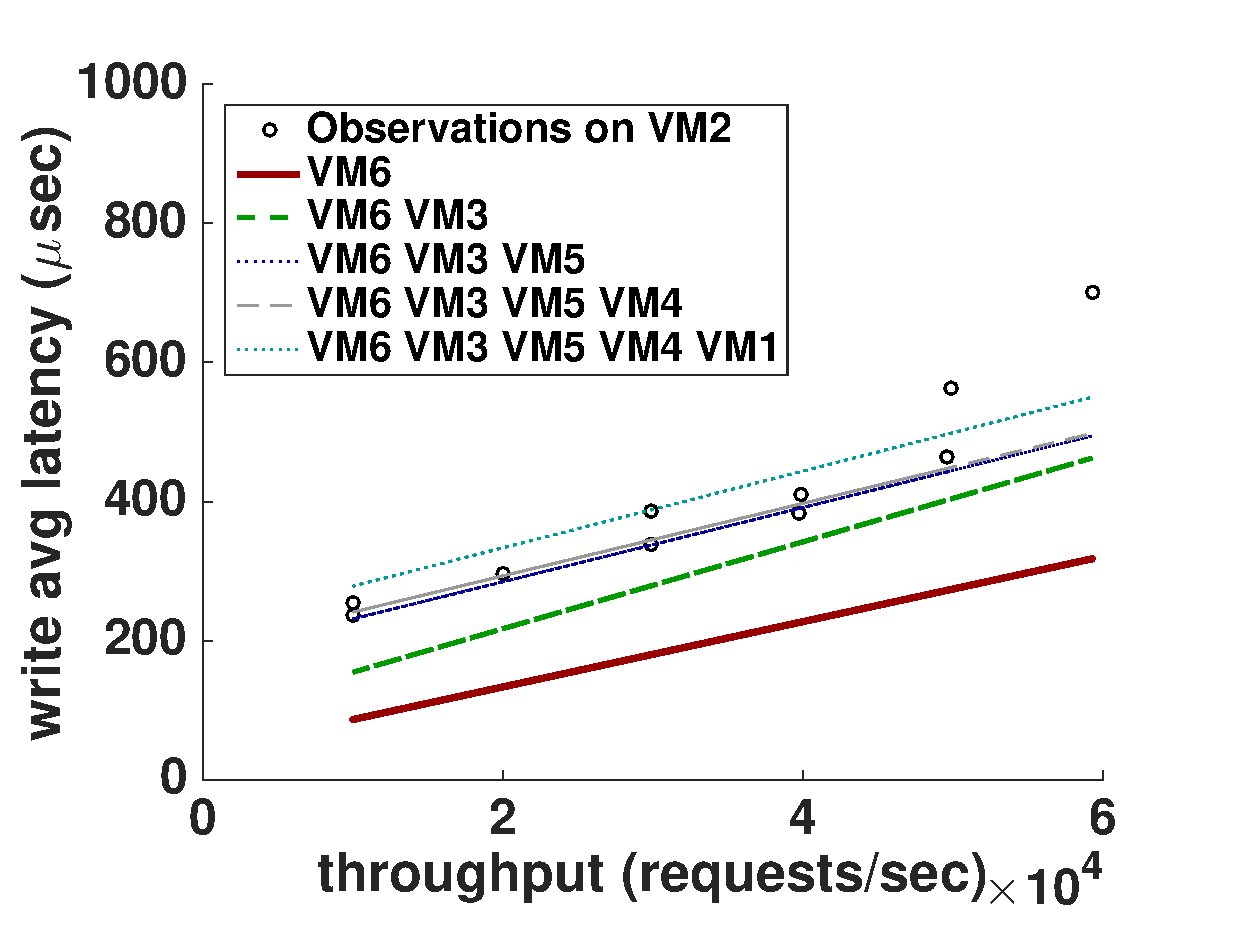
\includegraphics[width=0.45\textwidth]{fit_write_avg_latency_r3_2x_m3_2x_r3_x_r3__m3__m3_x.eps}
\caption{Redis average write latency vs throughput. ~\bu{TODO: cleanup plot formatting; make the numbers on the axes larger, label both the axes, use darker colors, move the box with names of providers to the top-left part of the graph.}}
\label{figure:redisbarread}
\end{figure}

\begin{figure}[htbp]
\centering	
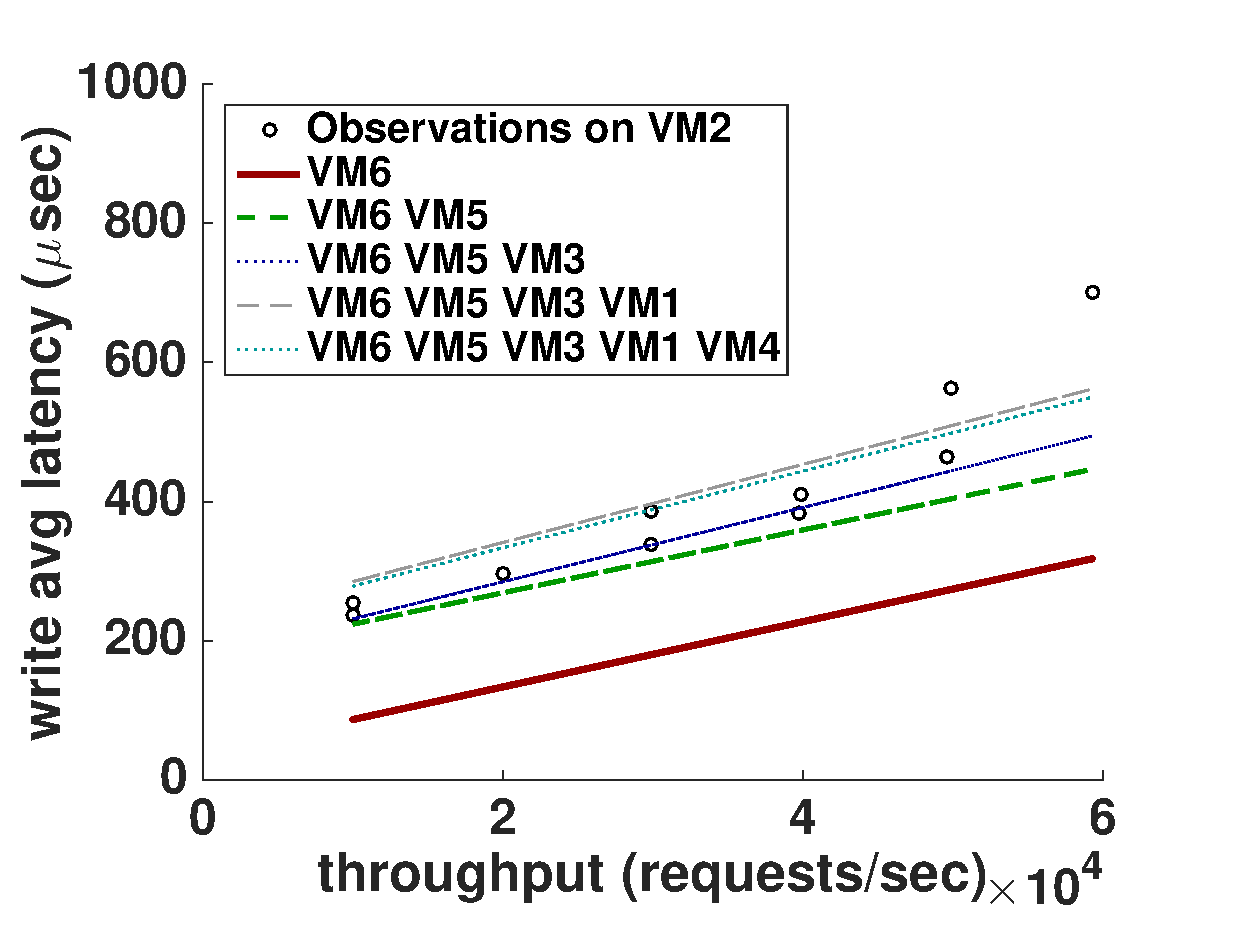
\includegraphics[width=0.45\textwidth]{fit_write_avg_latency_r3_2x_r3_x_m3_2x_m3__r3__m3_x.eps}
\caption{Redis average write latency vs throughput. ~\bu{TODO: cleanup plot formatting; make the numbers on the axes larger, label both the axes, use darker colors, move the box with names of providers to the top-left part of the graph.}}
\label{figure:redisbarread}
\end{figure}

\begin{figure}[htbp]
\centering	
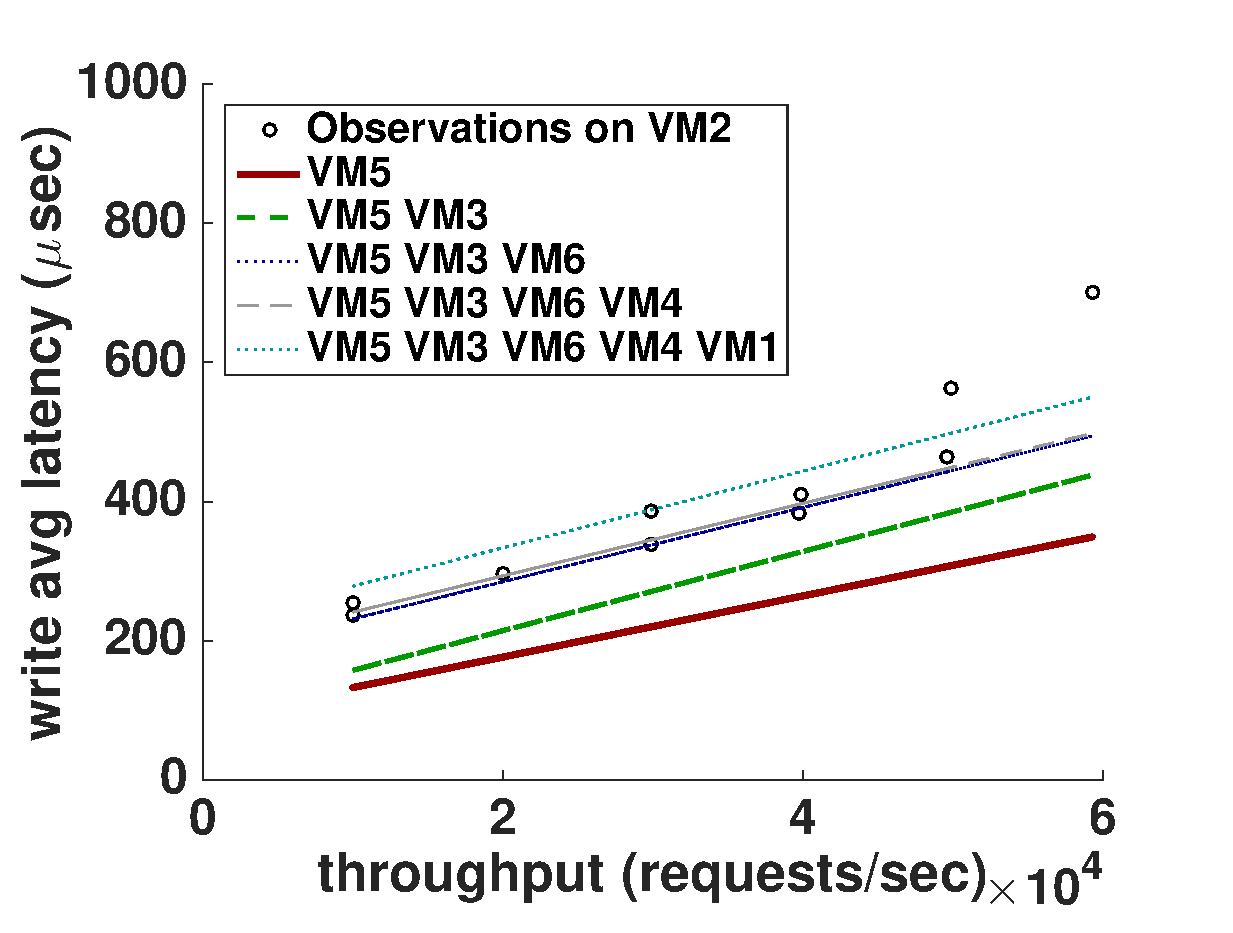
\includegraphics[width=0.45\textwidth]{fit_write_avg_latency_r3_x_m3_2x_r3_2x_r3__m3__m3_x.eps}
\caption{Redis average write latency vs throughput. ~\bu{TODO: cleanup plot formatting; make the numbers on the axes larger, label both the axes, use darker colors, move the box with names of providers to the top-left part of the graph.}}
\label{figure:redisbarread}
\end{figure}

\begin{figure}[htbp]
\centering	
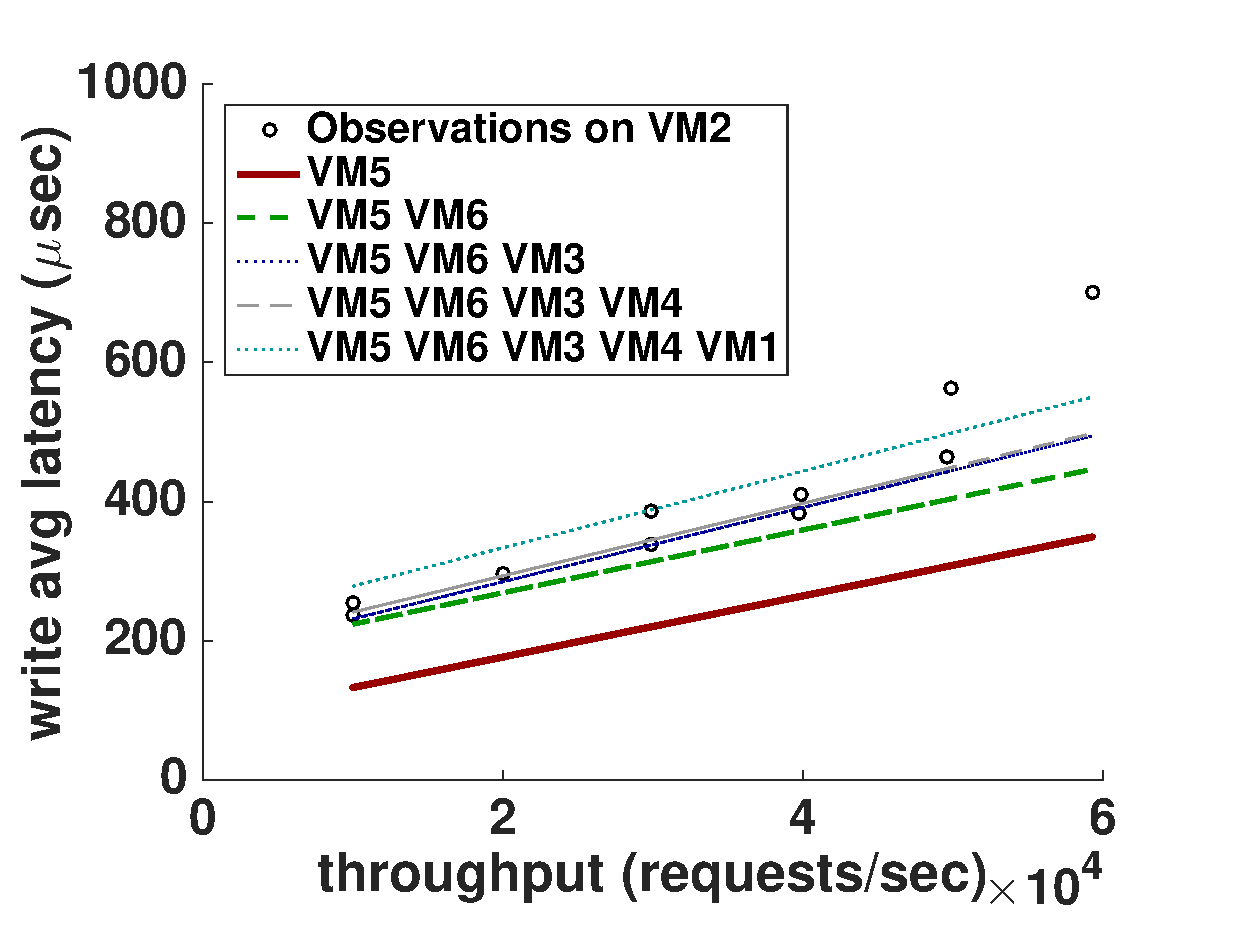
\includegraphics[width=0.45\textwidth]{fit_write_avg_latency_r3_x_r3_2x_m3_2x_r3__m3__m3_x.eps}
\caption{Redis average write latency vs throughput. ~\bu{TODO: cleanup plot formatting; make the numbers on the axes larger, label both the axes, use darker colors, move the box with names of providers to the top-left part of the graph.}}
\label{figure:redisbarread}
\end{figure}
\end{comment}

\begin{figure*}
\subfloat[]{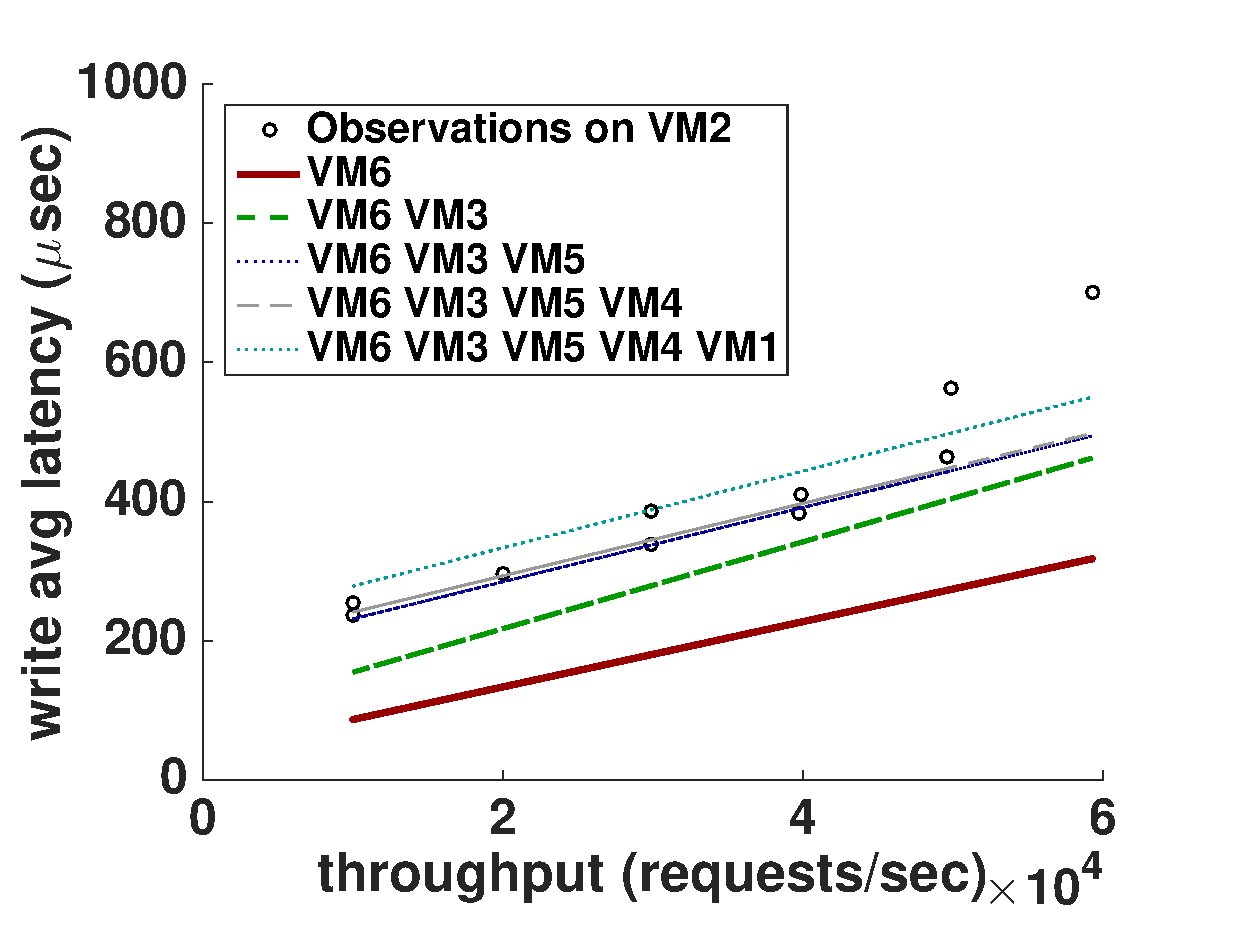
\includegraphics[width=0.5\textwidth]{fit_write_avg_latency_r3_2x_m3_2x_r3_x_r3__m3__m3_x.eps}} 
\subfloat[]{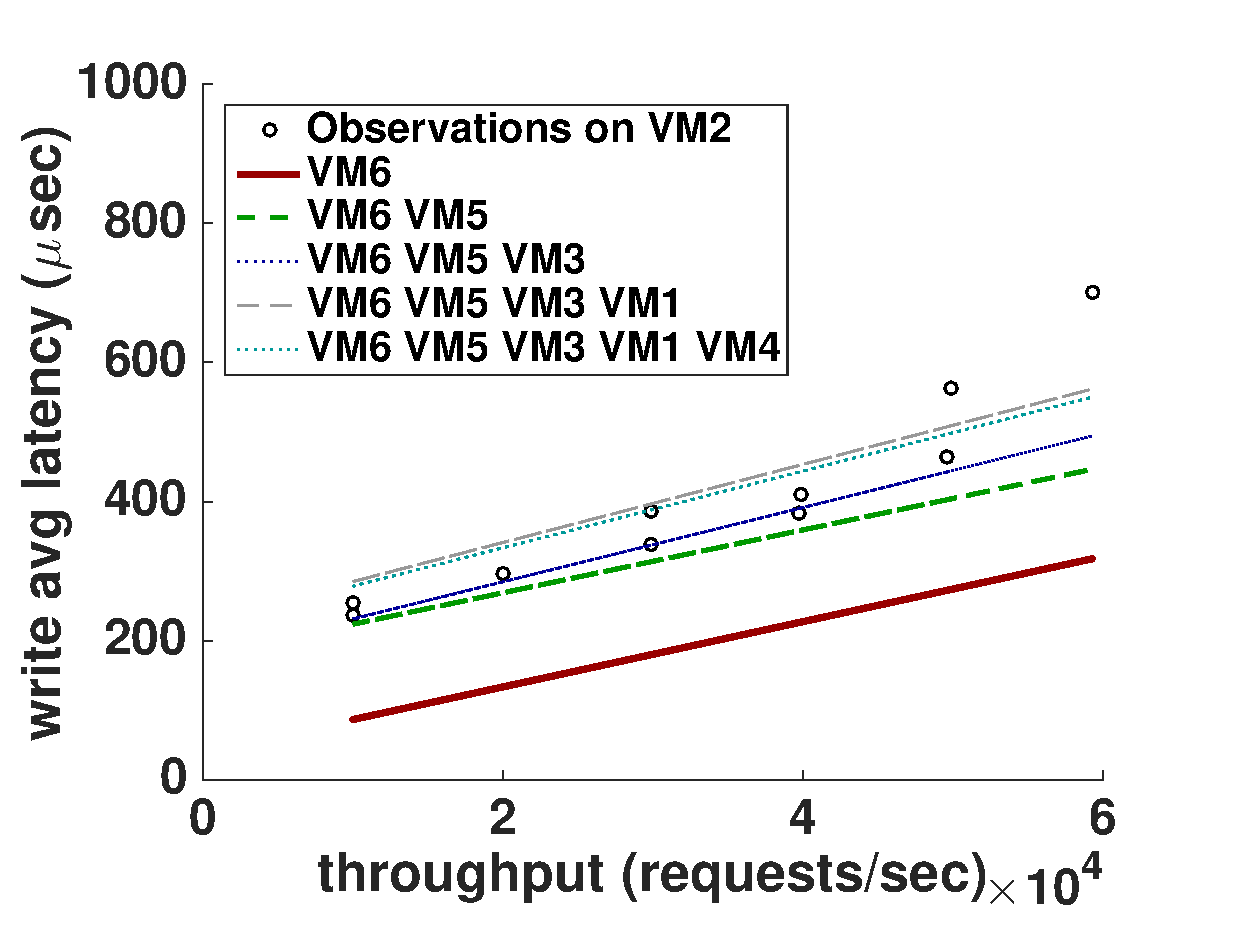
\includegraphics[width=0.5\textwidth]{fit_write_avg_latency_r3_2x_r3_x_m3_2x_m3__r3__m3_x.eps}}\\
\subfloat[]{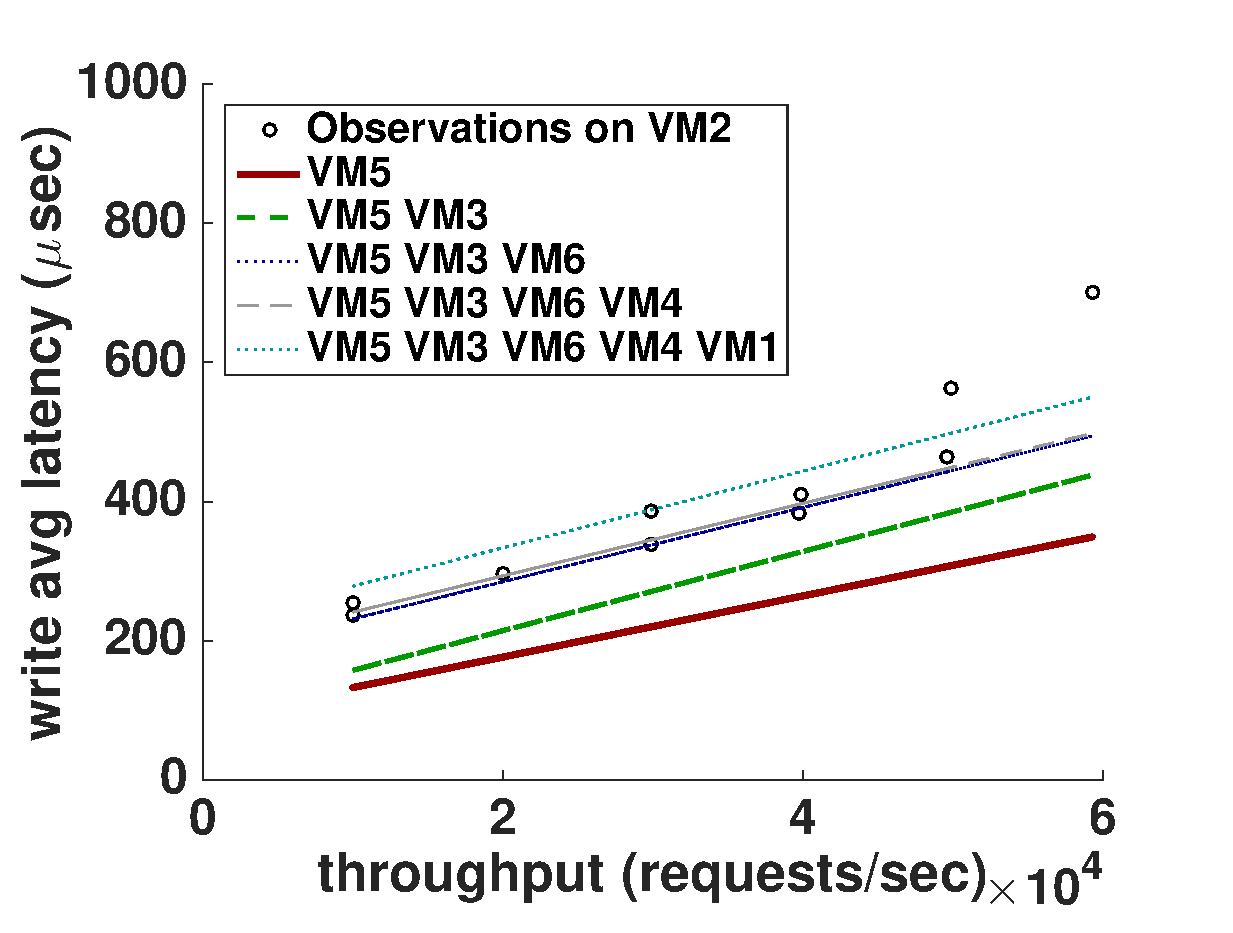
\includegraphics[width=0.5\textwidth]{fit_write_avg_latency_r3_x_m3_2x_r3_2x_r3__m3__m3_x.eps}}
\subfloat[]{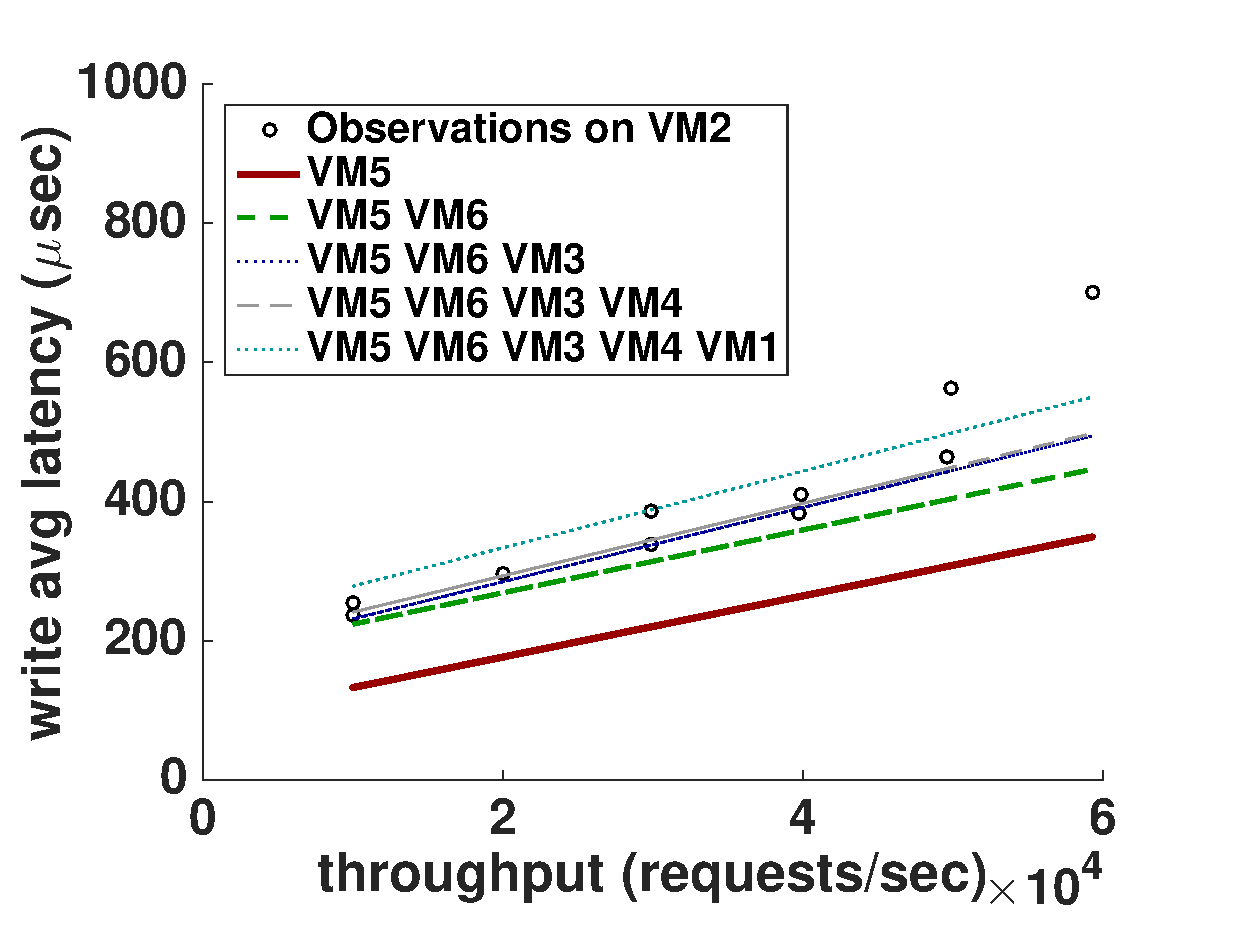
\includegraphics[width=0.5\textwidth]{fit_write_avg_latency_r3_x_r3_2x_m3_2x_r3__m3__m3_x.eps}} 
\caption{Prediction of Redis write latency on $VM_2$ compared for model calibration using a variety of training sets ranging in size from 1 to 5 VM types.}
\label{figure:redisfitwrite}
\end{figure*}

\subsection{Case Study 2: Apache Cassandra}
\vspace{10pt}

Apache Cassandra is a Table/Key-Value hybrid NoSQL database.  It is suitable for applications that require high availability provided by replication.  In terms of the CAP theorem, Cassandra prioritizes availability and performance over consistency, making it highly performant and scalable, though consistency is eventual rather than strong, for typical Cassandra applications. % We install Apache Cassandra was on Amazon EC2 instances of various VM instance types. 
We do our testing on Cassandra clusters with 5 nodes.  
We run our testing with a replication factor of three, so every database record is stored on three of the five nodes.  We report results when using weak (or eventual) consistency, using a consistency level of ``ONE.'' We find qualitatively similar results when repeating these experiments with Cassandra's strict consistency settings that we omit due to space constraints. 

For a sample VM type that we want to predict the performance of Cassandra, we select training sets of increasing size from the remaining VM types.  We select $VM_4$ for prediction, and do multiple linear regressions on the training set for sizes 1 through 5 for read latency and write latency data.  We observe that every time another VM type is added to the training set, the associated $R^2_{predicted}$ improves for $VM_4$ for both read and write latency (see representative results in Table \ref{table:cassandra1} and Table \ref{table:cassandra2}).

These findings are also presented in an alternative way in Figure \ref{figure:cassandrabarread}, %and Figure \ref{figure:cassandrabarwrite}, 
where we plot histograms of $R^2_{predicted}$ to emphasize the improved fit associated with larger training sets of VM types.  The x-axis is labeled with sets of numbers of those VM types in each training set.

Finally, Figure \ref{figure:cassandrafitread} shows multiple linear fits offered by several training sets and shows the progressive improvement of the  model for for read latency for Cassandra as the training set grows. Figure \ref{figure:cassandrafitwrite} shows the same for write latency. We conclude that our evaluation offers supporting evidence for our second case study. 


\begin{comment}
  \begin{figure}
  \centering
    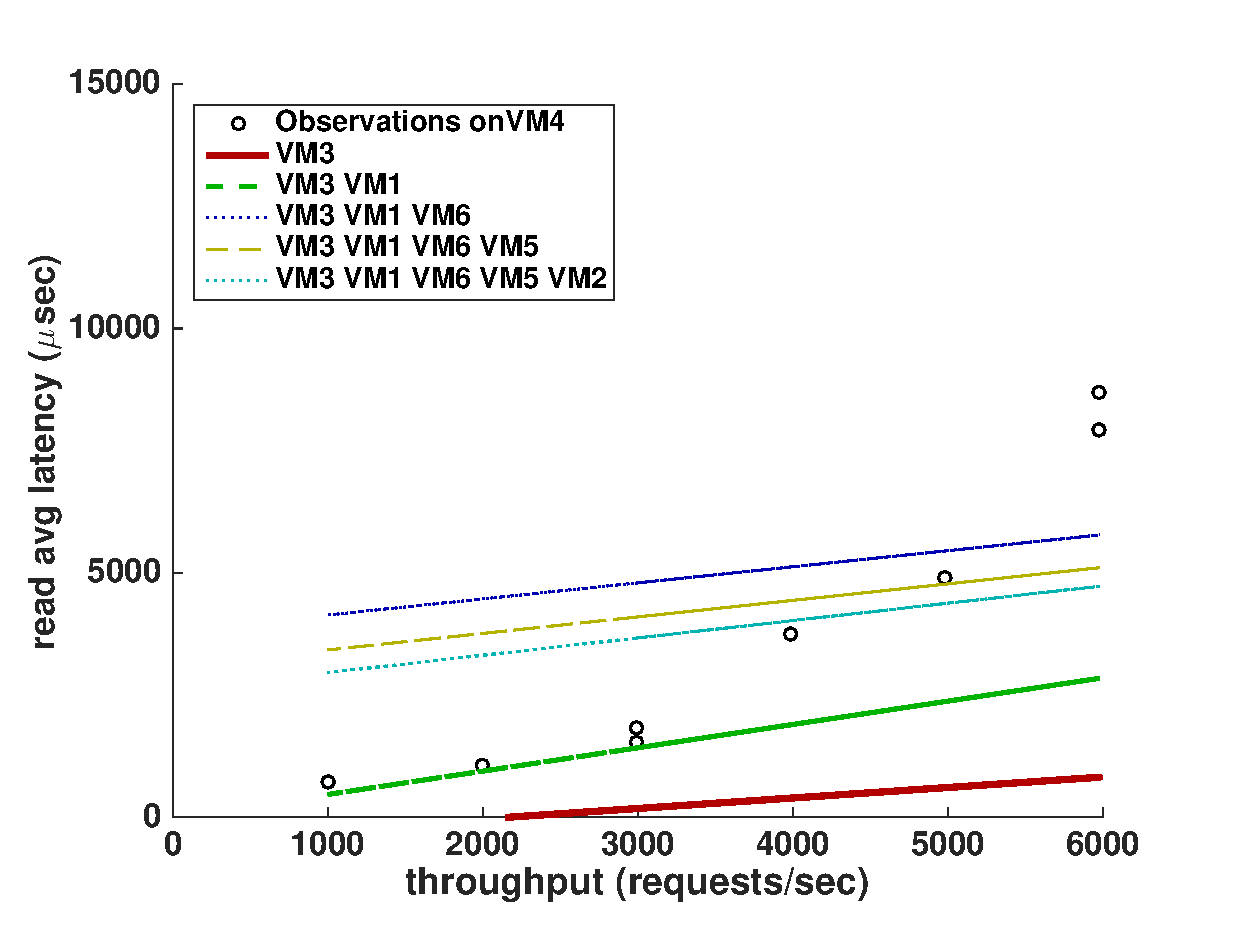
\includegraphics[scale = 0.25]{cassandra_fit_read_avg_latency_m3_2x_m3__r3_2x_r3_x_m3_x_r3_.eps}
    \caption{Cassandra average read latency vs throughput}
    \label{figure:redisbarread}
  \end{figure}

  \begin{figure}
  \centering
    \includegraphics[scale = 0.25]{cassandra_fit_read_avg_latency_r3_2x_r3_x_m3_x_m3__m3_2x_r3_.eps}
    \caption{Cassandra average read latency vs throughput}
    \label{figure:redisbarread}
  \end{figure}

  \begin{figure}
  \centering
    \includegraphics[scale = 0.25]{cassandra_fit_read_avg_latency_r3__m3_x_r3_2x_m3_2x_r3_x_m3_.eps}
    \caption{Cassandra average read latency vs throughput}
    \label{figure:redisbarread}
  \end{figure}

  \begin{figure}
  \centering
    \includegraphics[scale = 0.25]{cassandra_fit_read_avg_latency_r3_x_m3__r3_2x_m3_x_m3_2x_r3_.eps}
    \caption{Cassandra average read latency vs throughput}
    \label{figure:redisbarread}
  \end{figure}
\end{comment}

  \begin{figure}
    \centering
    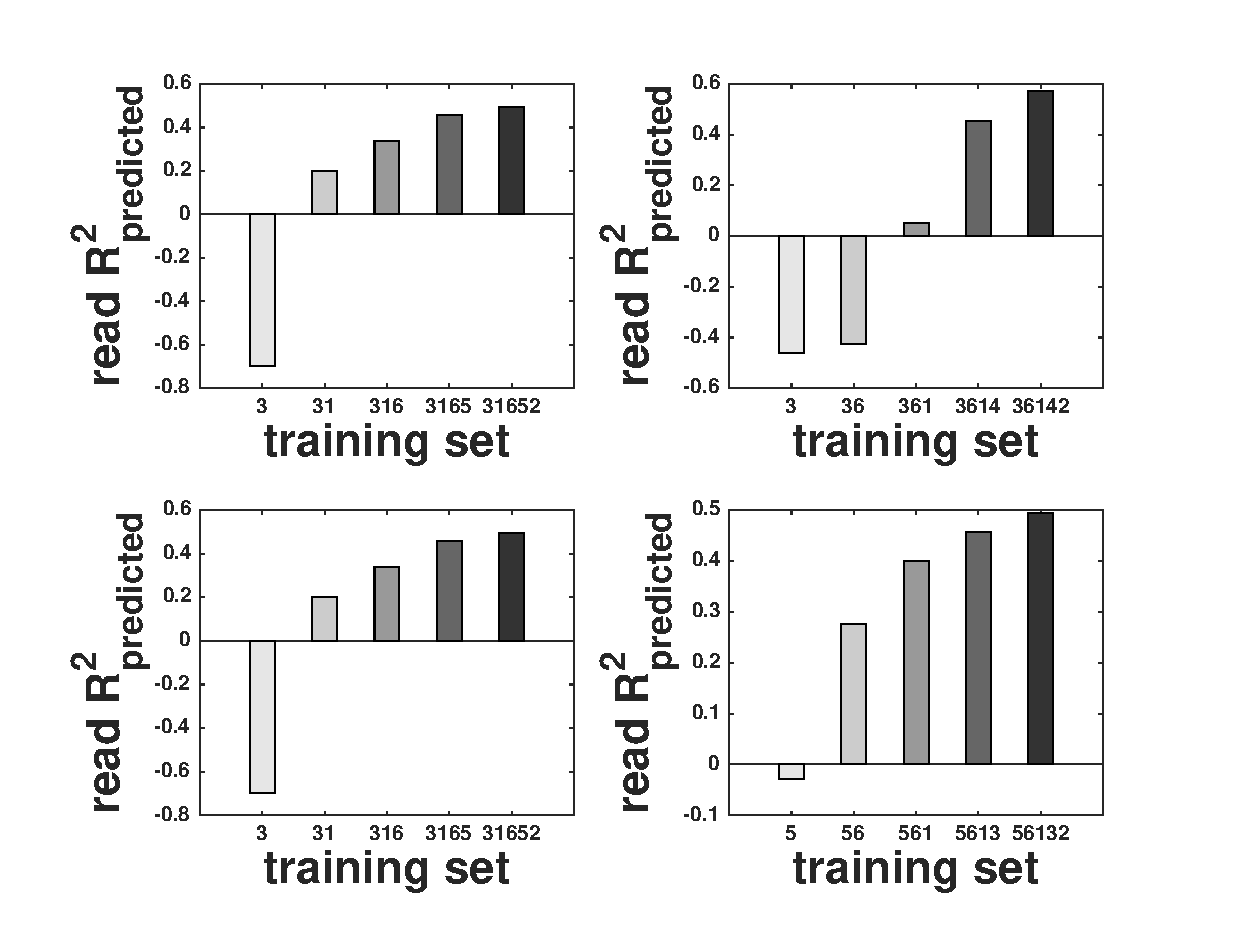
\includegraphics[scale = 0.4]{cassandra_bar_read_avg_latency.eps}
    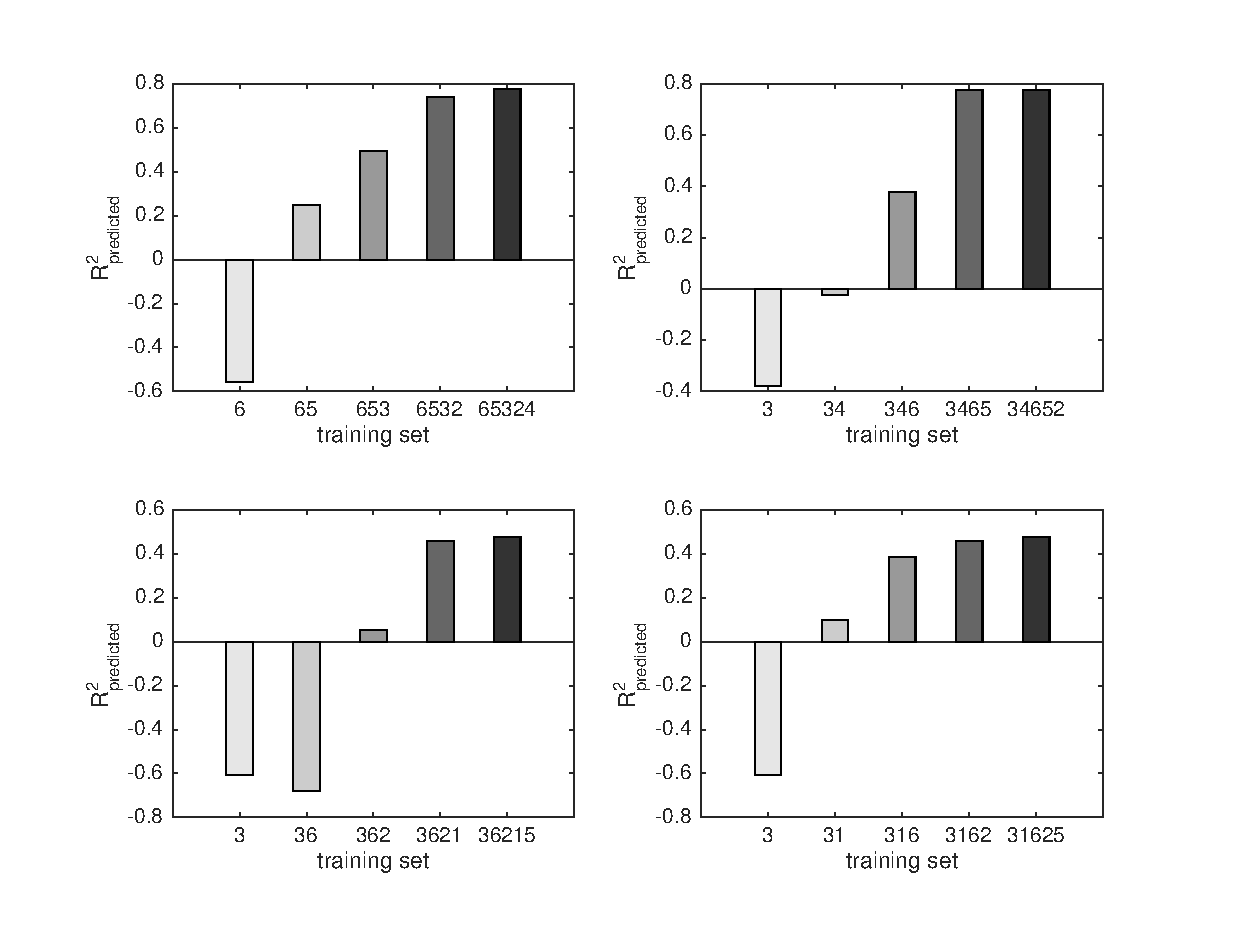
\includegraphics[scale = 0.4]{cassandra_bar_write_avg_latency.eps}
    \caption{Cassandra read and write $R^2_{predicted}$ vs training set. We find that $R^2_{predicted}$ improves consistency with more diverse training sets for a wide range of training set choices supporting our basic hypothesis.}
    \label{figure:cassandrabarread}
  \end{figure}

%   \begin{figure}
%     \centering
    
%     \caption{Cassandra write $R^2_{predicted}$ vs training set}
%     \label{figure:cassandrabarwrite}
%   \end{figure}

\begin{figure*}
\subfloat[]{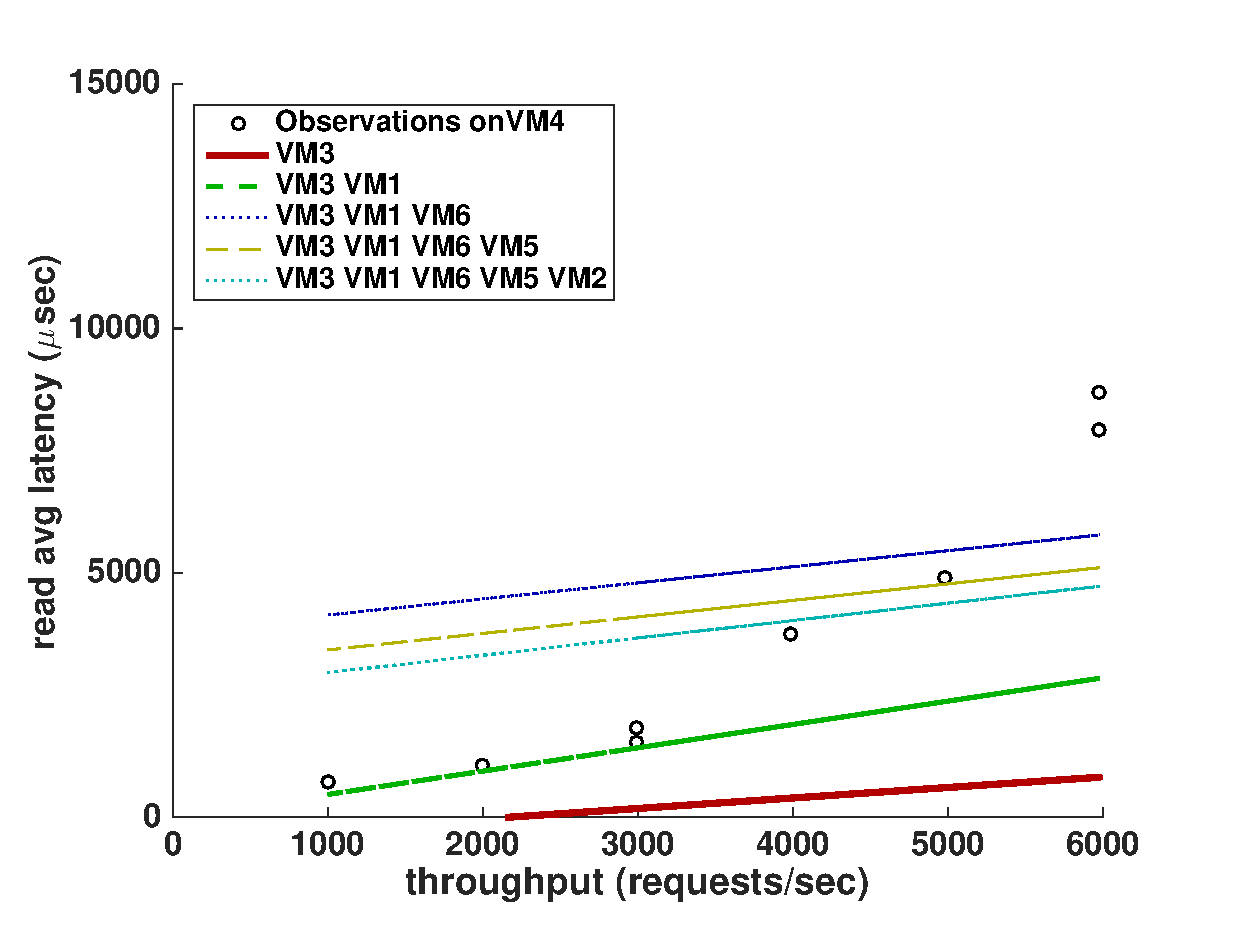
\includegraphics[width=0.25\textwidth]{cassandra_fit_read_avg_latency_m3_2x_m3__r3_2x_r3_x_m3_x_r3_.eps}} 
\subfloat[]{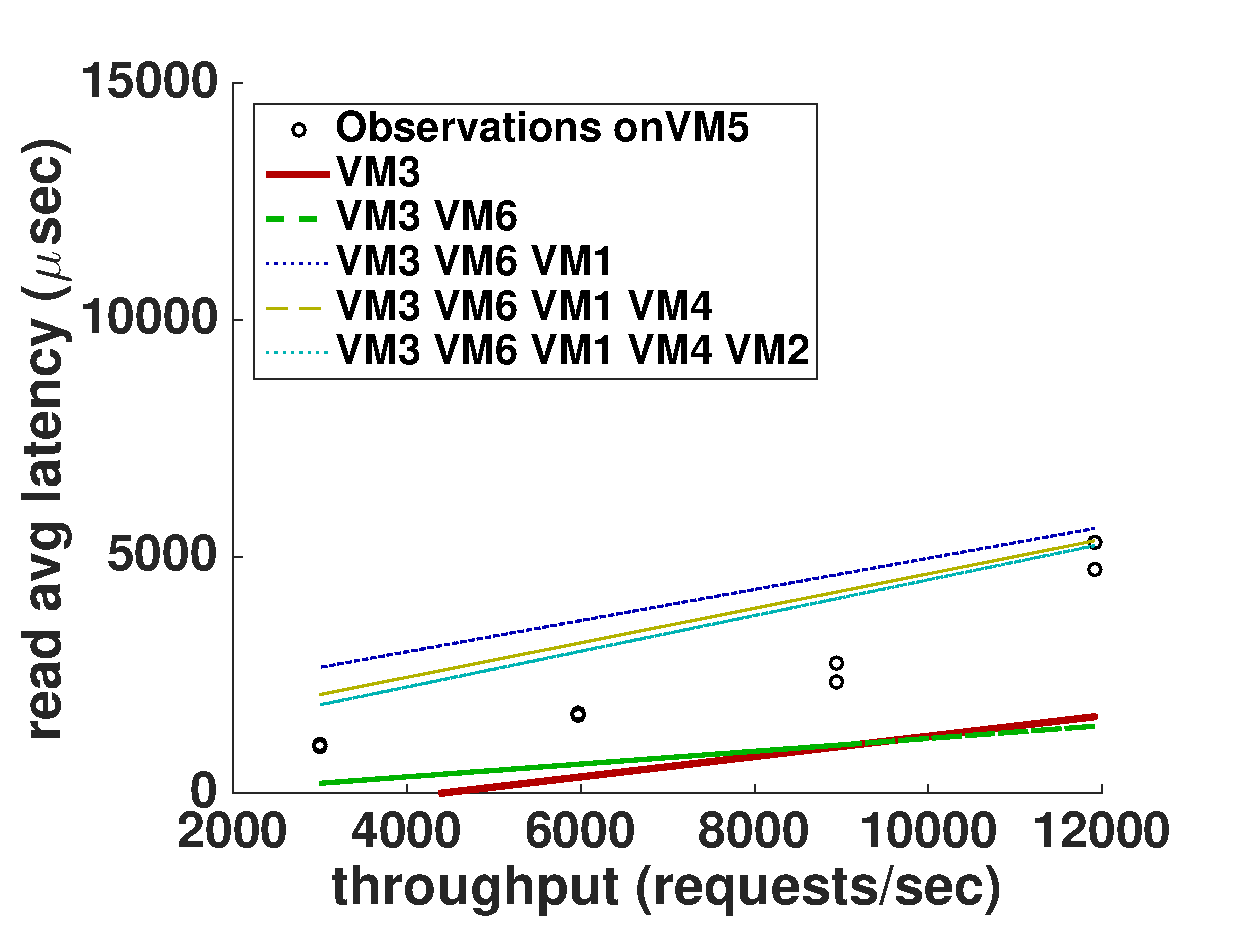
\includegraphics[width=0.25\textwidth]{cassandra_fit_read_avg_latency_m3_2x_r3_2x_m3__r3__m3_x_r3_x.eps}}
\subfloat[]{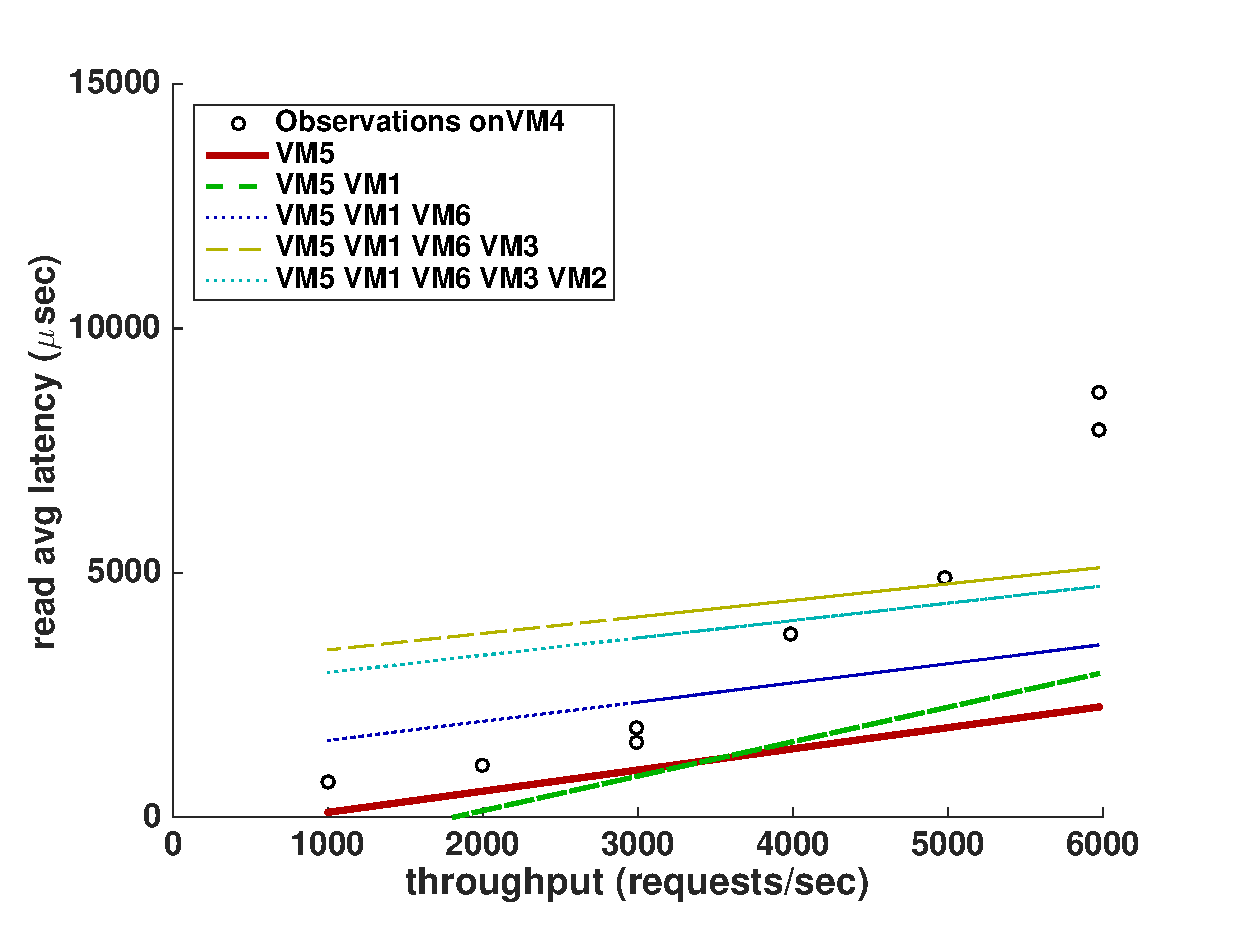
\includegraphics[width=0.25\textwidth]{cassandra_fit_read_avg_latency_r3_x_m3__r3_2x_m3_2x_m3_x_r3_.eps}}
\subfloat[]{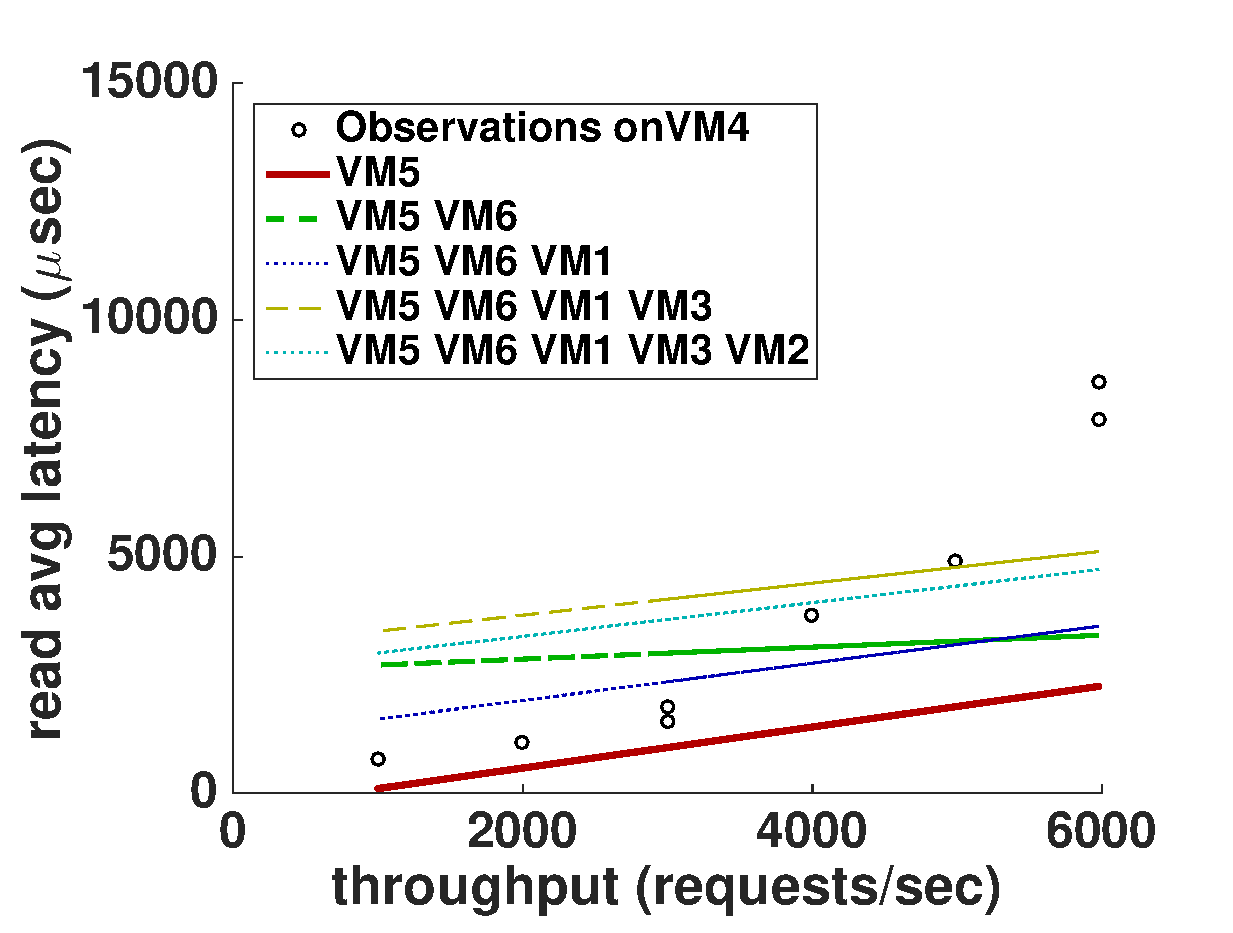
\includegraphics[width=0.25\textwidth]{cassandra_fit_read_avg_latency_r3_x_r3_2x_m3__m3_2x_m3_x_r3_.eps}}
\caption{Prediction of Cassandra read latency on $VM_4$ compared for model calibration using a variety of training sets ranging in size from 1 to 5 VM types.}
\label{figure:cassandrafitread}
\end{figure*}

\begin{comment}
  \begin{figure}
  \centering
    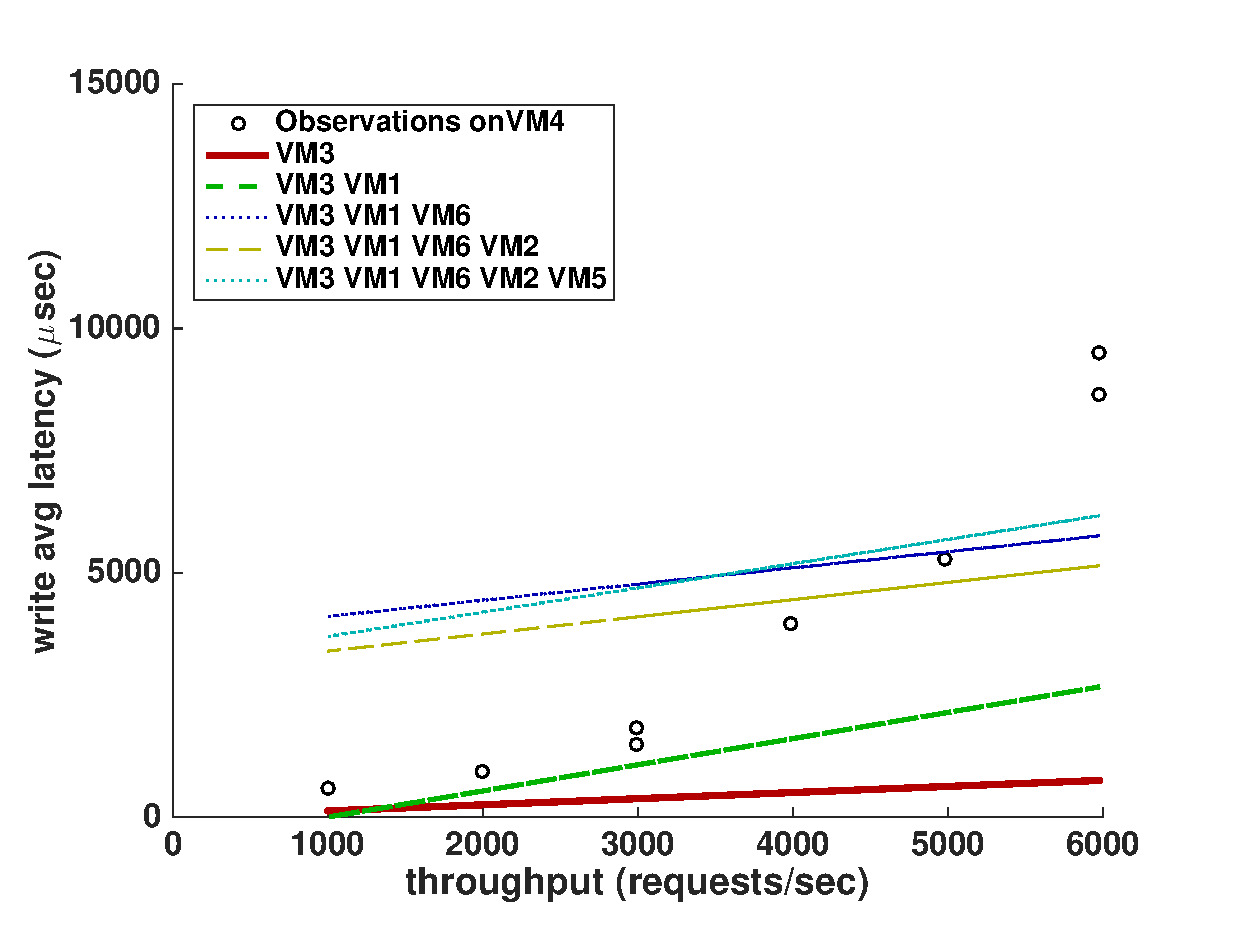
\includegraphics[scale = 0.25]{cassandra_fit_write_avg_latency_m3_2x_m3__r3_2x_m3_x_r3_x_r3_.eps}
    \caption{Cassandra average read latency vs throughput}
    \label{figure:redisbarread}
  \end{figure}

  \begin{figure}
  \centering
    \includegraphics[scale = 0.25]{cassandra_fit_write_avg_latency_m3_2x_m3_x_r3__r3_2x_r3_x_m3_.eps}
    \caption{Cassandra average read latency vs throughput}
    \label{figure:redisbarread}
  \end{figure}

  \begin{figure}
  \centering
    \includegraphics[scale = 0.25]{cassandra_fit_write_avg_latency_m3_2x_r3_x_r3_2x_m3_x_r3__m3_.eps}
    \caption{Cassandra average write latency vs throughput}
    \label{figure:redisbarread}
  \end{figure}

  \begin{figure}
  \centering
    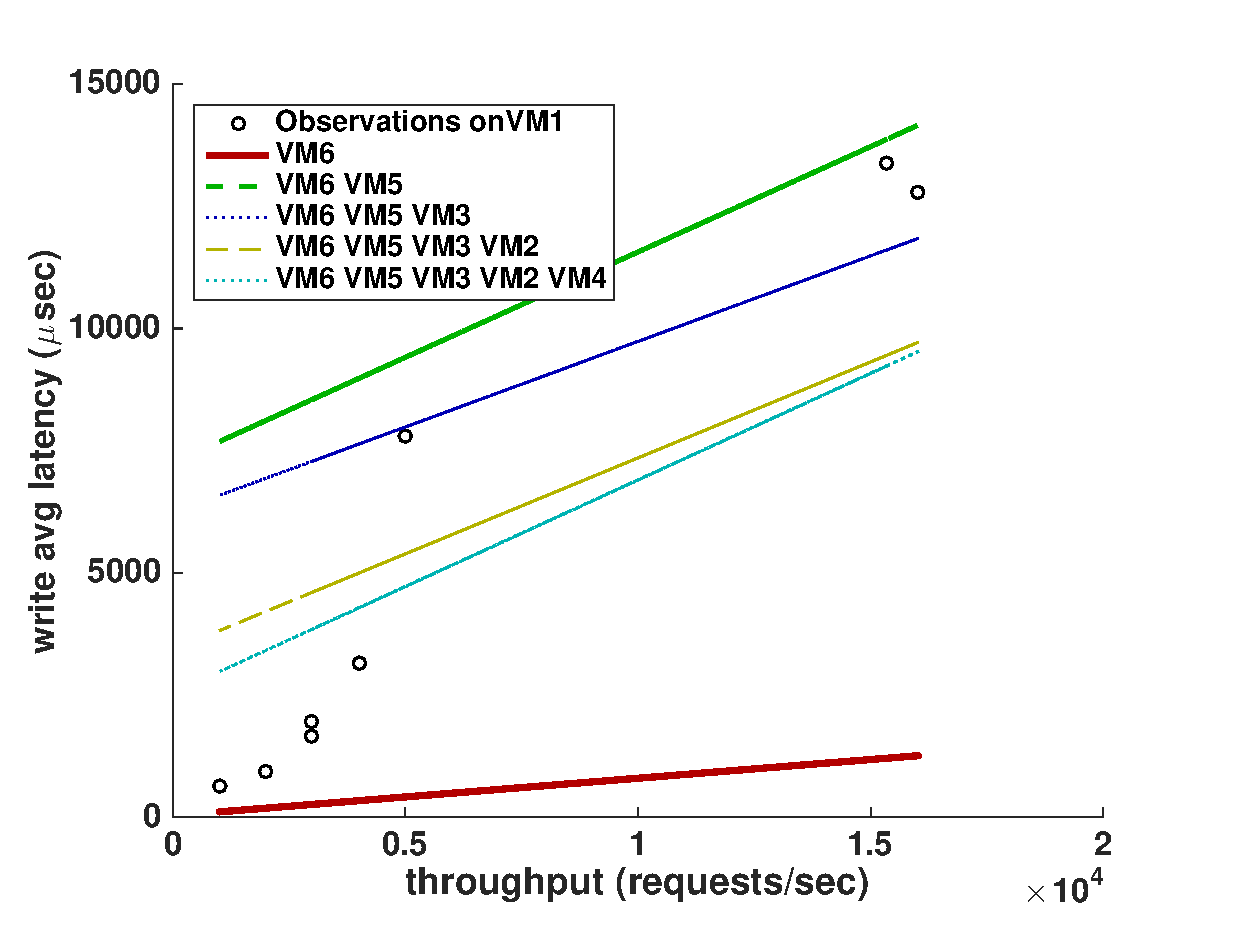
\includegraphics[scale = 0.25]{cassandra_fit_write_avg_latency_r3_2x_r3_x_m3_2x_m3_x_r3__m3_.eps}
    \caption{Cassandra average write latency vs throughput}
    \label{figure:redisbarread}
  \end{figure}
\end{comment}


\begin{figure*}
\subfloat[]{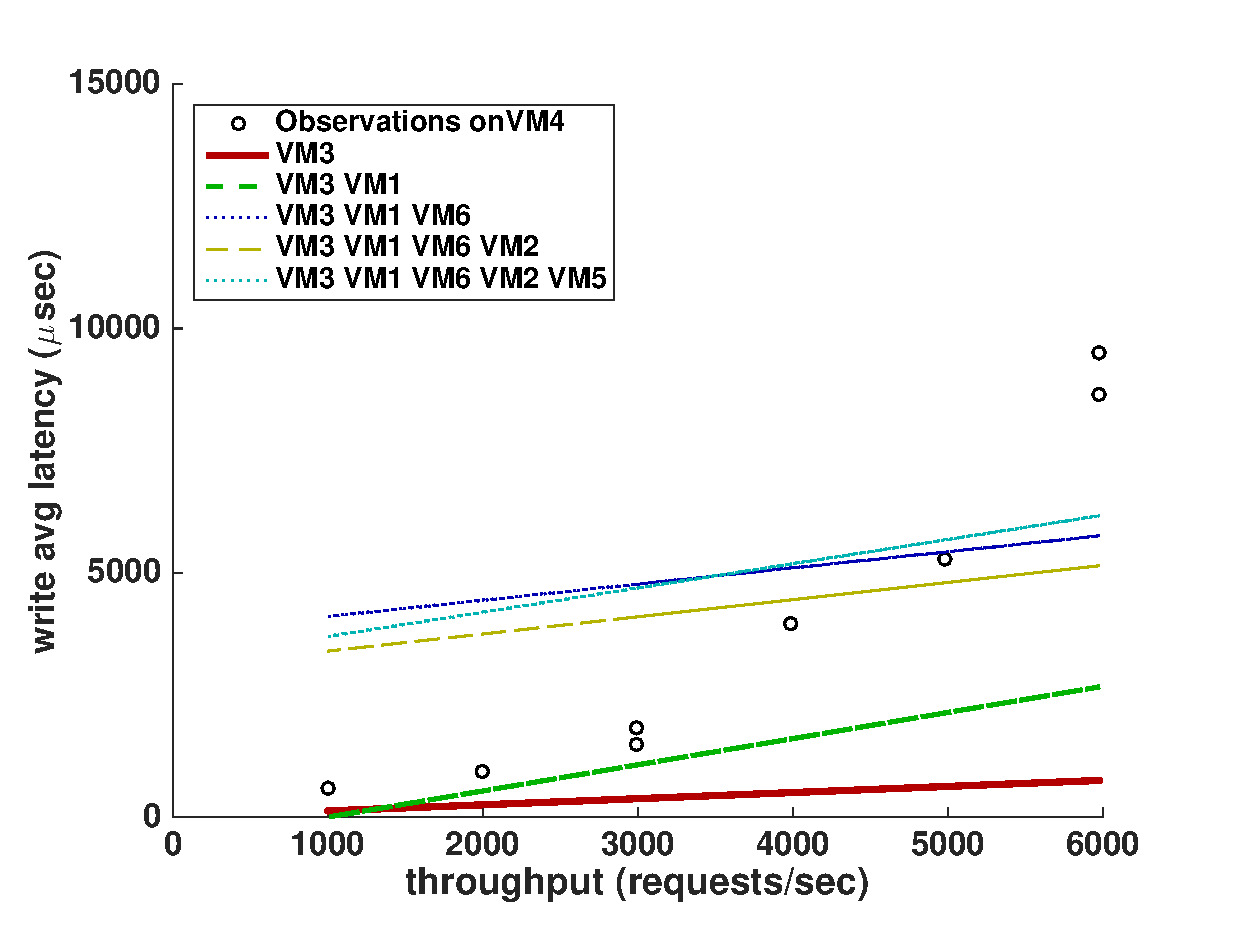
\includegraphics[width=0.25\textwidth]{cassandra_fit_write_avg_latency_m3_2x_m3__r3_2x_m3_x_r3_x_r3_.eps}} 
\subfloat[]{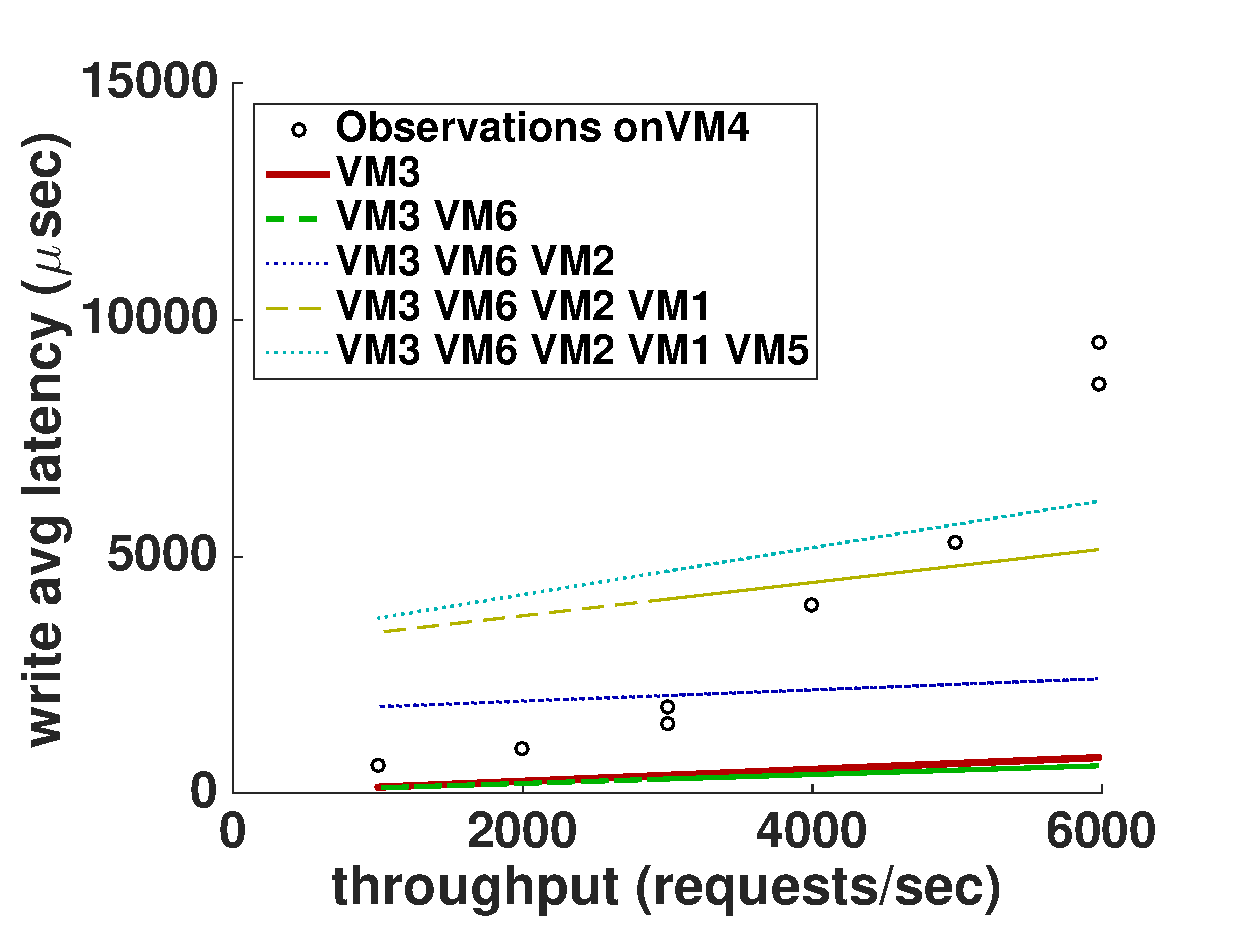
\includegraphics[width=0.25\textwidth]{cassandra_fit_write_avg_latency_m3_2x_r3_2x_m3_x_m3__r3_x_r3_.eps}}
\subfloat[]{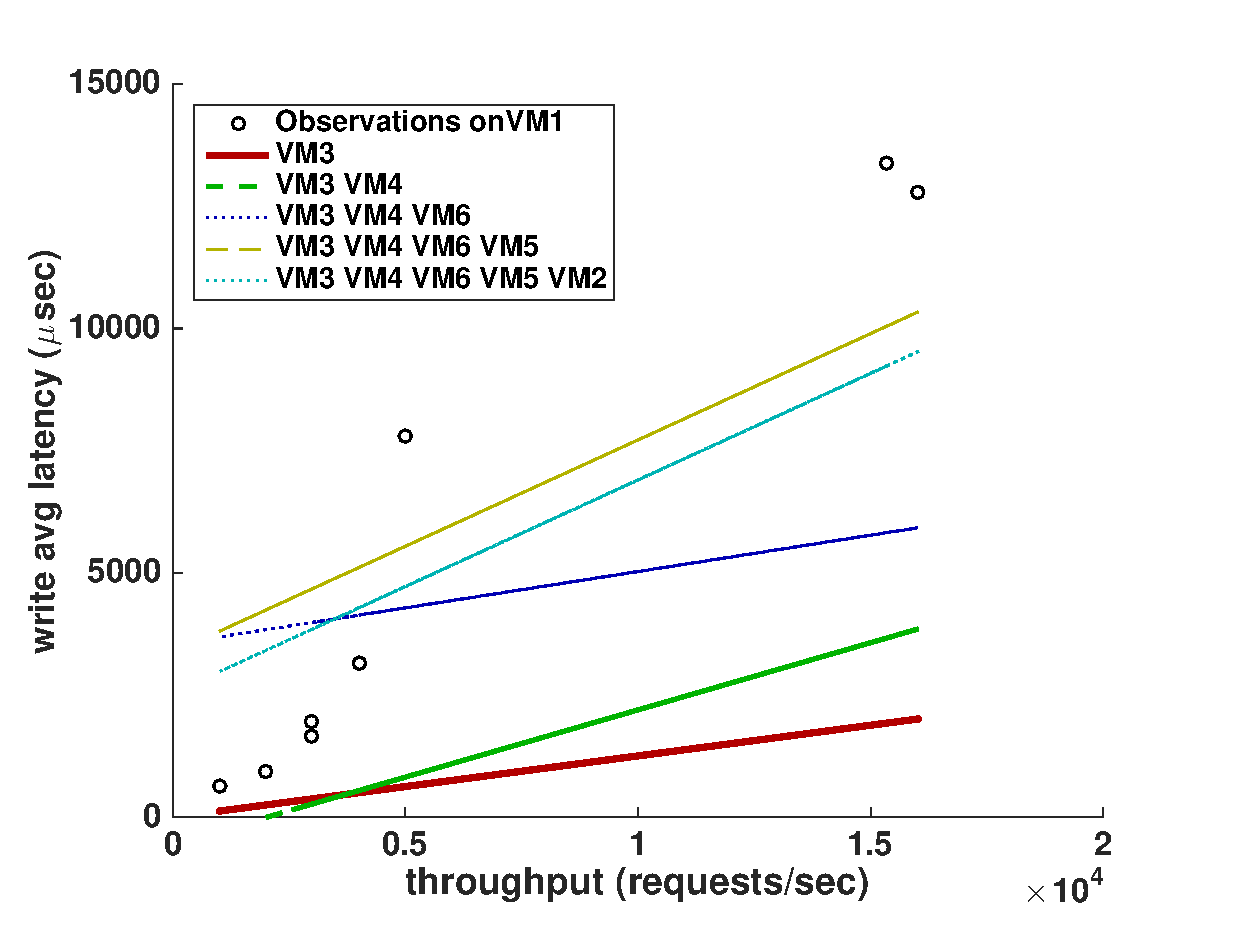
\includegraphics[width=0.25\textwidth]{cassandra_fit_write_avg_latency_m3_2x_r3__r3_2x_r3_x_m3_x_m3_.eps}}
\subfloat[]{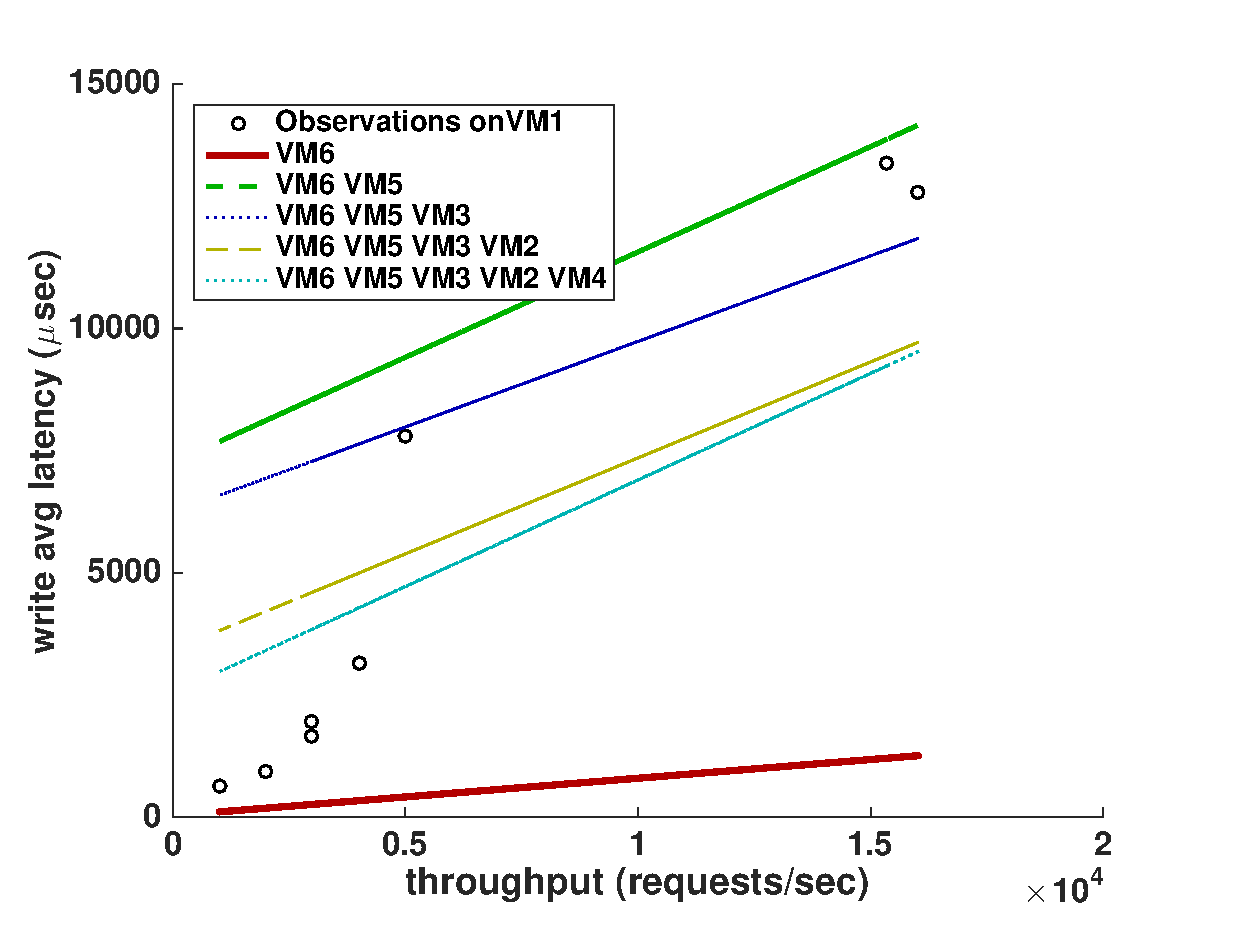
\includegraphics[width=0.25\textwidth]{cassandra_fit_write_avg_latency_r3_2x_r3_x_m3_2x_m3_x_r3__m3_.eps}} 
\caption{Prediction of Cassandra write latency on $VM_4$ compared for model calibration using a variety of training sets ranging in size from 1 to 5 VM types.}
\label{figure:cassandrafitwrite}
\end{figure*}

% \subsubsection{Evaluation for a Weak Consistency Configuration}

% consistency=ONE

% Workload B (95/5 r/w) with uniform distribution

% Present data for
% 3 VM types: gen,mem,cpu, throughputs 5000-20000, replication factor 3, 5 nodes

\begin{table}
\centering
\caption{Cassandra $R_{predicted}^2$ for $VM_4$}
\begin{tabular}{|r|r|l|} \hline
$R_{read}^2$&$R_{write}^2$&Training Data\\ \hline
-0.699345 & -0.559334  & VM3 \\ \hline 
0.199993 & 0.249826  & VM3 VM1 \\ \hline 
0.337298 &  0.495004 & VM3 VM1 VM6 \\ \hline 
0.456502 & 0.741173  & VM3 VM1 VM6 VM5 \\ \hline 
0.49455 & 0.776169  & VM3 VM1 VM6 VM5 VM2 \\ \hline 
\hline\end{tabular}
\label{table:cassandra1}
% \end{table}

% \begin{table}
\centering
\caption{Cassandra $R_{predicted}^2$ for $VM_5$}
\begin{tabular}{|r|r|l|} \hline
$R_{read}^2$&$R_{write}^2$&Training Data\\ \hline
-0.462405 & -0.380705  & VM3 \\ \hline 
-0.425988 &  -0.0225972 & VM3 VM6 \\ \hline 
0.053444 &  0.379236 & VM3 VM6 VM1 \\ \hline 
0.453755 & 0.775494  & VM3 VM6 VM1 VM4 \\ \hline 
0.574078 & 0.776169  & VM3 VM6 VM1 VM4 VM2 \\ \hline 
\hline\end{tabular}
\label{table:cassandra2}
% \end{table}

% \begin{table}
\centering
\caption{Cassandra $R_{predicted}^2$ for $VM_4$}
\begin{tabular}{|r|r|l|} \hline
$R_{read}^2$&$R_{write}^2$&Training Data\\ \hline
-0.0293728 & -0.605137  & VM5 \\ \hline 
0.157659 &  -0.681656 & VM5 VM1 \\ \hline 
0.400541 & 0.0545588  & VM5 VM1 VM6 \\ \hline 
0.456502 & 0.459396  & VM5 VM1 VM6 VM3 \\ \hline 
0.49455 & 0.477652  & VM5 VM1 VM6 VM3 VM2 \\ \hline 
\hline\end{tabular}
\label{table:cassandra3}
% \end{table}

% \begin{table}
\centering
\caption{Cassandra $R_{predicted}^2$ for $VM_4$}
\begin{tabular}{|r|r|l|} \hline
$R_{read}^2$&$R_{write}^2$&Training Data\\ \hline
-0.0293728 & -0.605137  & VM5 \\ \hline 
0.276549 & 0.0974061  & VM5 VM6 \\ \hline 
0.400541 & 0.385513  & VM5 VM6 VM1 \\ \hline 
0.456502 &  0.459396 & VM5 VM6 VM1 VM3 \\ \hline 
0.49455 &  0.477652 & VM5 VM6 VM1 VM3 VM2 \\ \hline 
\hline\end{tabular}
\label{table:cassandra4}
\end{table}

\subsection{Case Study 3: MySQL}
\vspace{10pt}

%\mm{

MySQL is an extremely popular ACID SQL database server, the backbone of numerous commercial applications.  For our testing we deployed MySQL %was deployed 
using Amazon Relational Database Service (Amazon RDS)~\cite{amazon-rds}, which abstracts away the deployment and administration of OS and relationship database software.  We benchmark MySQL %was tested 
on the six VM types listed in Table \ref{table:awstypes}.  %Unlike for the previous case studies, we test using YCSB Workload A (50\% read, 50\% write) with a uniform distribution.

The MySQL data shows a higher variation in latency than our other case studies, and our linear regression model does not fit it as well as it does the previous two applications. %did not a linear regression as well as the first two.  
We show a sample %Example 
result for MySQL in Figure \ref{figure:mysql}. We do continue to see that the model accuracy as captured by $R^2_{predicted}$ does continue to improve with the addition of more VM types to the training set, although the value of $R^2_{predicted}$ is lower than observed for Redis and Cassandra. 

This may be due to the higher write latency of SQL databases, or possibly something with Amazon's RDS architecture that made our YCSB testing method unsuitable.  Another possibility is that the network availability for RDS varies over time, making consistent results harder to reproduce. This requires further investigation that forms part of our future work. Despite these inadequacies in our modeling, however, the basic expectation we have regarding the role of diversity does appear to hold. 
%}

  \begin{figure}
    \centering
    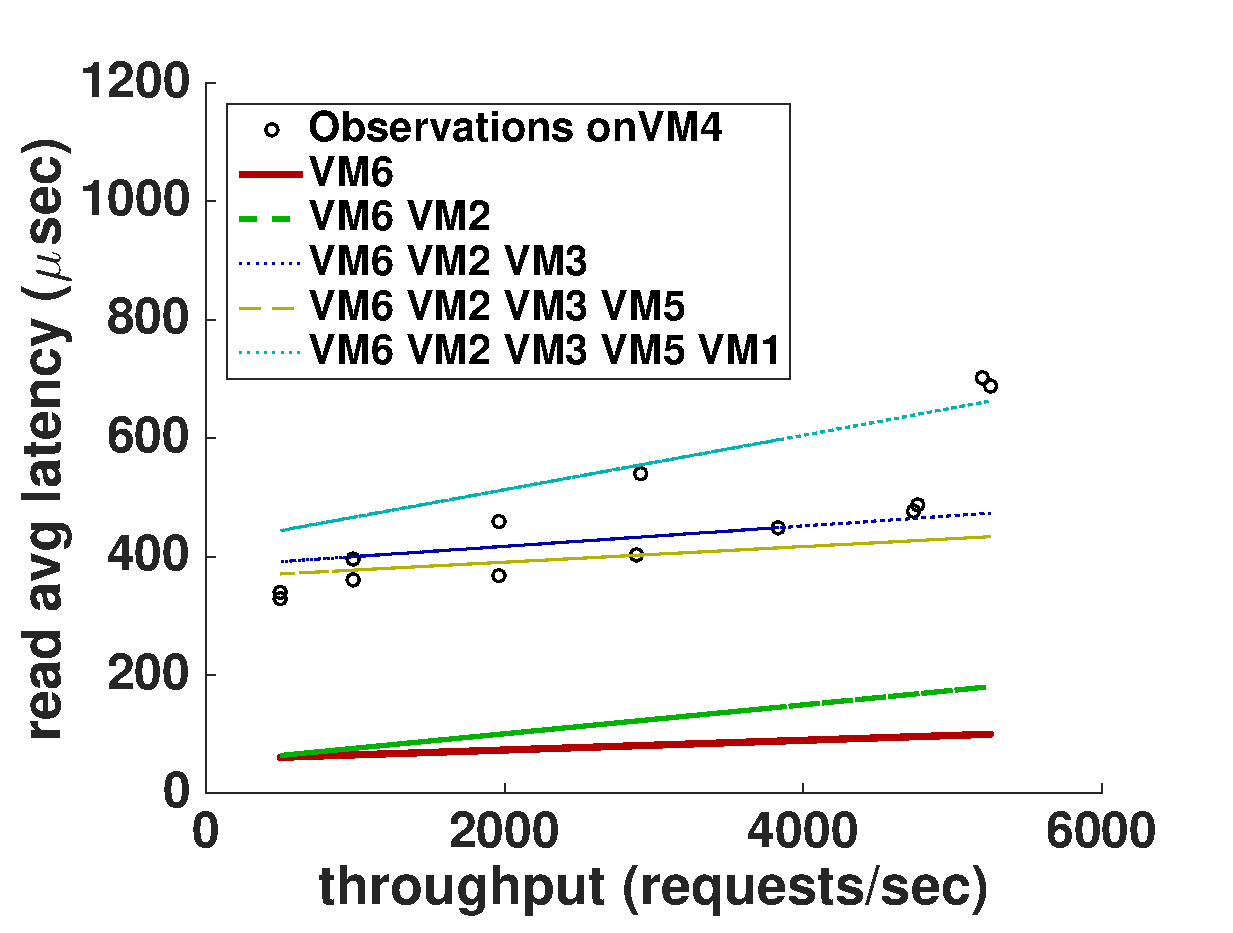
\includegraphics[scale = 0.4]{mysql_fit_read_avg_latency.eps}
    \caption{Read latency/throughput plot for MySQL. Although our multiple linear regression model offers a poorer prediction for MySQL than for our other case studies, we continue to observe an improvement in its efficacy upon increasing the diversity of the training set. }
    \label{figure:mysql}
  \end{figure}

\begin{comment}
  \begin{figure}
    \centering
    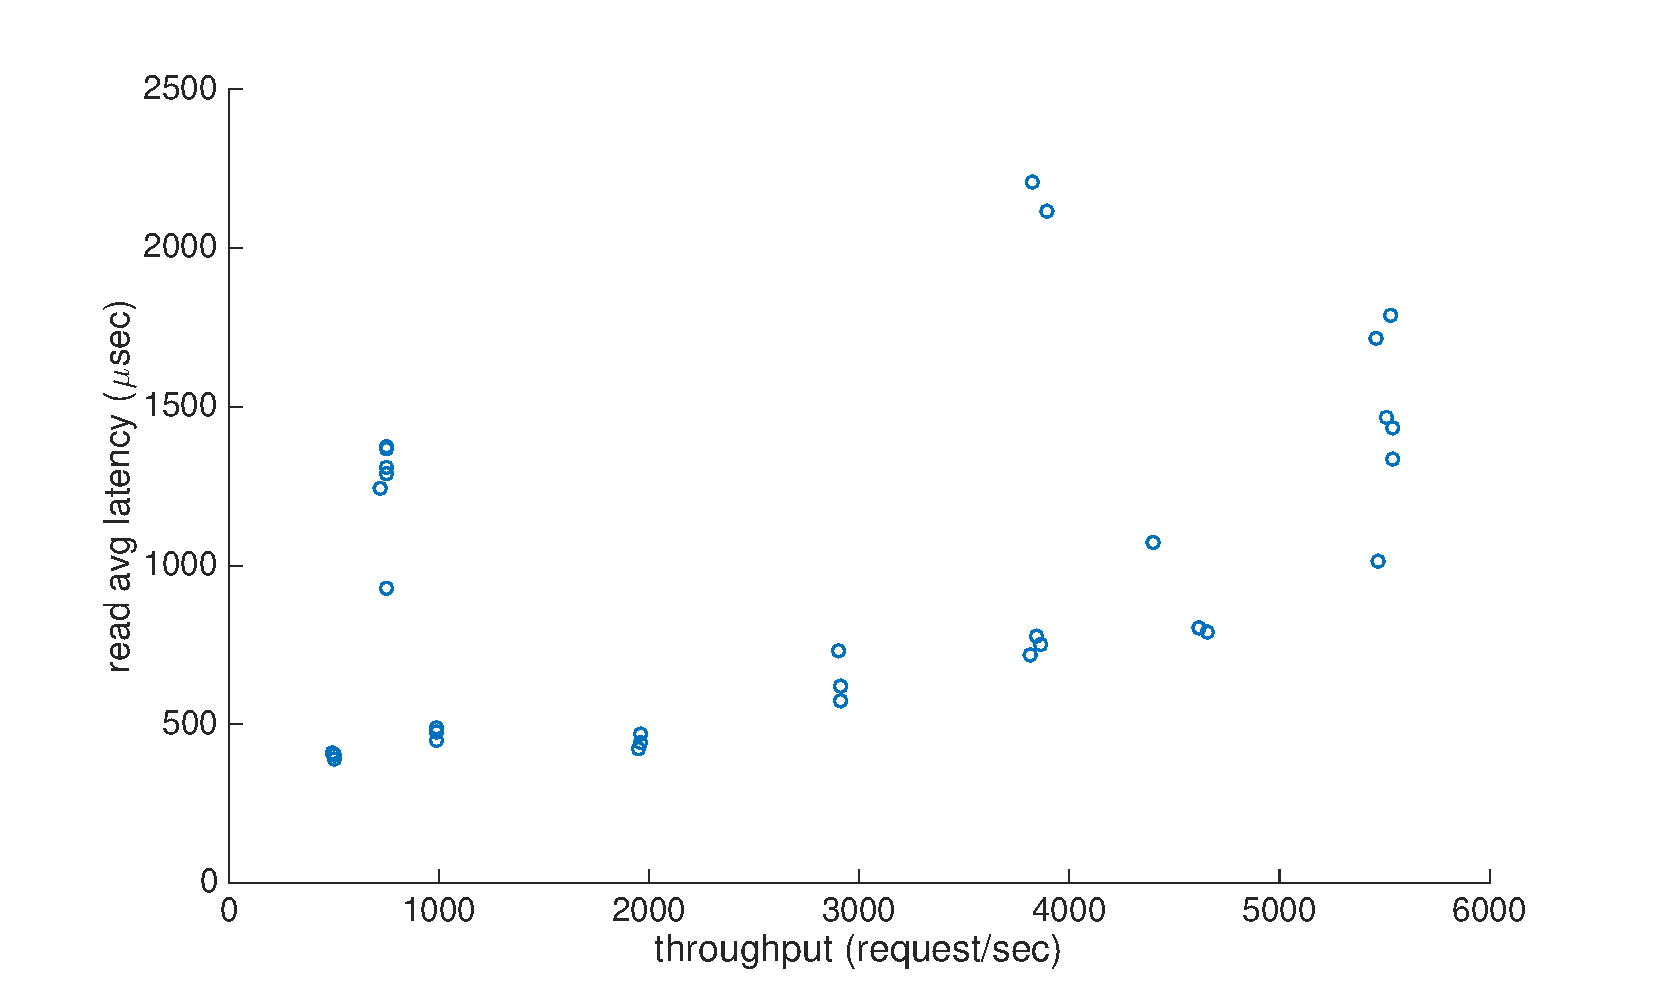
\includegraphics[scale = 0.3]{mysql.eps}
    \caption{Read latency/throughput plot for MySQL}
    \label{figure:mysql}
  \end{figure}
\end{comment}

% \begin{table}
% \centering
% \caption{MySQL $R_{predicted}^2$ for $VM_6$}
% \begin{tabular}{|r|r|l|} \hline
% $R_{read}^2$&$R_{write}^2$&Training Data\\ \hline
% 0 & 0& $VM_1,VM_2,VM_3$\\ \hline
% 0 & 0& $VM_1,VM_2,VM_3,VM_4$\\ \hline
% 0 & 0& $VM_1,VM_2,VM_3,V_4,V_5$\\ \hline
% \hline\end{tabular}
% \label{table:mysql}
% \end{table}
